%
\edef\maxSat{MAX-SAT}%
\edef\maxTSat{MAX-3SAT}%
\def\oFlip{\ensuremath{1}-flip}%
\def\tFlip{\ensuremath{2}-flip}%
\def\mFlip{\ensuremath{m}-flip}%
%
\section{Example: \maxSat}%
%
%%
\gdef\maxSatClauses{\textcolor{red}{\ensuremath{k}}}%
\gdef\maxSatVariables{\textcolor{green}{\ensuremath{n}}}%
\gdef\maxSatVariable{\ensuremath{x}}%
\gdef\maxSatVariablei#1{\ensuremath{\maxSatVariable_{#1}}}%
\gdef\maxSatFormula{\ensuremath{B}}%
%%
\begin{frame}%
\frametitle{MAX-SAT}%
~\\%
\begin{itemize}%
\item Satisfiability Problems (SAT)\uncover<2->{:%
\begin{itemize}
\item The satisfiability problem (SAT) is one of the most prominent problems in artificial intelligence, logic, theoretical computer science, and various application areas.\scitep{HS2000SAORFROS}%
\item<3-> Given: formula \maxSatFormula\ in Boolean logic consisting of \maxSatVariables\ Boolean variables $\vec{\maxSatVariable}=(\maxSatVariablei{1}, \maxSatVariablei{2}, \dots, \maxSatVariablei{\maxSatVariables})^T$ which each can be either \texttt{true} or \texttt{false}%
\item<4-> Goal: find a setting for these variables so that $\maxSatFormula$ becomes \texttt{true}%
\item<5-> \maxSatFormula\ consists of \maxSatClauses\ clauses which are combined with \inQuotes{$\land$}%
\end{itemize}%
}%
%
\item<6-> MAX-SAT\uncover<7->{%
\begin{itemize}%
\item SAT turned into an optimization problem\scitep{HS2005SLSFAA}%
\item<7-> candidate solution: bit string of length \maxSatVariables\ holding the value of each variable%
\item<8-> make as many clauses become \texttt{true} as possible%
\item<9-> minimize objective function $\objectiveFunctionb{\vec{x}} = \textnormal{number of clauses which are \texttt{false}}$%
\item<10-> $\objectiveFunctionb{\vec{x}}=0$ $\Longrightarrow$ all clauses are \texttt{true}, SAT problem solved%
\item<11-> $\objectiveFunctionb{\vec{x}}=\maxSatClauses$ $\Longrightarrow$ all clauses are \texttt{false}%
\end{itemize}%
}%
%
\end{itemize}%
\end{frame}%
%
\begin{frame}[t]%
\frametitle{Investigated Algorithms}%
\begin{itemize}%
\item We want to compare the performance of six algorithms\uncover<2->{:%
\begin{enumerate}%
\item 1-flip Hill Climber%
\item<2-> 1-flip Hill Climber with Restarts%
\item<3-> 2-flip Hill Climber%
\item<4-> 2-flip Hill Climber with Restarts
\item<5-> $m$-flip Hill Climber
\item<6-> $m$-flip Hill Climber with Restarts%
%
\end{enumerate}%
}%
\item<7-> \alert{Which of these algorithms performs best? When? Why?}%
\end{itemize}%
\end{frame}%
%
\begin{frame}%
\frametitle{Benchmark}%
\begin{itemize}%
\item As benchmark, we use \emph{some} instances from \satLib\expandafter\scitep{\satLibReferences}\uncover<2->{:%
\begin{center}%
\medskip%
\begin{small}%
\begin{tabular}{|l|r|r||l|r|r|}%
\hline%
\textbf{Instance Set} & \textbf{\ensuremath{\mathbf{\maxSatVariables}}} & \textbf{\ensuremath{\mathbf{\maxSatClauses}}}&\textbf{Instance Set} & \textbf{\ensuremath{\mathbf{\maxSatVariables}}} & \textbf{\ensuremath{\mathbf{\maxSatClauses}}}\\%
\hline%
\texttt{uf020}&20&91&\texttt{uf150}&150&645\\%
\texttt{uf050}&50&218&\texttt{uf175}&175&753\\%
\texttt{uf075}&75&325&\texttt{uf200}&200&860\\%
\texttt{uf100}&100&430&\texttt{uf225}&225&960\\%
\texttt{uf125}&125&538&\texttt{uf250}&250&1065\\%
\hline%
\end{tabular}%
\medskip%
\end{small}%
\end{center}%
}%
\item<3-> We pick the first ten instances from each set, i.e., test 100 instances in total%
\item<4-> All instances are satisfiable%
\item<5-> The problem instances have the following features\uncover<6->{:%
\begin{itemize}%
\item \maxSatVariables: the number of variables%
\item<7-> \maxSatClauses: the number of clauses (related to \maxSatVariables)%
\end{itemize}%
}%
\end{itemize}%
\end{frame}%
%
%
\begin{frame}%
\frametitle{Experiments}%
\begin{itemize}%
\item Now we want to do the experiments.%
\item<2-> What data shall we collect?\uncover<3->{%
\begin{enumerate}%
\item Data should allow us to reproduce algorithm progress over time%
\item<4-> We can collect one data point whenever the algorithm makes an improvement in terms of \objectiveFunction\uncover<5->{ (and one at the end of run)}%
\item<6-> $\maxSatClauses+1$ possible objective values $\Longrightarrow$ at most $\maxSatClauses+2$ log points%
\item<7-> In each log point we record\uncover<8->{%
\begin{itemize}%
\item the number of function evaluations (\measureFEs) performed%
\item<9-> the elapsed runtime \measureRuntime\ (in \nano\second)%
\item<10-> the best objective value \measureObjectiveValue\ achieved so far%
\end{itemize}%
}%
\end{enumerate}%
}%
\end{itemize}%
\end{frame}%
%
%
\begin{frame}[t]%
\frametitle{Example of Log File}%
%
\begin{itemize}%
\item Example log file obtained from applying the 2-flip Hill Climber with Restarts to the 2\textsuperscript{nd} benchmark instance of set \texttt{uf075}.%
\end{itemize}%
%
\begin{locateBox}{0.25}{0.235}
\begin{listingBlock}[0.65]{Log File \texttt{uf075-02\_2FlipHCrs\_01.txt}.}
\centering
\begin{scaledBox}{!}{0.3\paperheight}
\lstinputlisting[tabsize=17]{graphics/maxsat_example/exampleMaxSatLogFile.txt}
\end{scaledBox}
\end{listingBlock}
\end{locateBox}
%
\begin{locateBox}[2-]{0}{0}
\begin{pgfpicture}%
\pgfpathrectangle{\pgfpoint{0pt}{0pt}}{\pgfpoint{\paperwidth}{\paperheight}}%
\pgfusepath{use as bounding box,clip}%
%
\pgfsetcolor{blue}%
\pgftext[right,bottom,at=\pgfpoint{0.2\paperwidth}{0.55\paperheight}]{log point}%
\pgfsetlinewidth{1pt}%
\pgfpathmoveto{\pgfpoint{0.21\paperwidth}{0.56\paperheight}}%
\pgfpathlineto{\pgfpoint{0.32\paperwidth}{0.525\paperheight}}%
\pgfusepath{stroke}%
\pgfsetlinewidth{2pt}%
\pgfpathrectangle{\pgfpoint{0.32\paperwidth}{0.51\paperheight}}{\pgfpoint{0.52\paperwidth}{0.03\paperheight}}%
\pgfusepath{stroke}%
%
\uncover<3->{%
%
\pgfsetcolor{red}%
\pgftext[right,bottom,at=\pgfpoint{0.2\paperwidth}{0.45\paperheight}]{ellapsed \measureFEs}%
\pgfsetlinewidth{1pt}%
\pgfpathmoveto{\pgfpoint{0.21\paperwidth}{0.46\paperheight}}%
\pgfpathlineto{\pgfpoint{0.36\paperwidth}{0.4\paperheight}}%
\pgfusepath{stroke}%
\pgfsetlinewidth{2pt}%
\pgfpathrectangle{\pgfpoint{0.36\paperwidth}{0.085\paperheight}}{\pgfpoint{0.1\paperwidth}{0.585\paperheight}}%
\pgfusepath{stroke}%
%
\uncover<4->{%
\pgfsetcolor{green}%
\pgftext[right,bottom,at=\pgfpoint{0.2\paperwidth}{0.35\paperheight}]{runtime [\nano\second]}%
\pgfsetlinewidth{1pt}%
\pgfpathmoveto{\pgfpoint{0.21\paperwidth}{0.365\paperheight}}%
\pgfpathlineto{\pgfpoint{0.56\paperwidth}{0.3\paperheight}}%
\pgfusepath{stroke}%
\pgfsetlinewidth{2pt}%
\pgfpathrectangle{\pgfpoint{0.56\paperwidth}{0.085\paperheight}}{\pgfpoint{0.11\paperwidth}{0.585\paperheight}}%
\pgfusepath{stroke}%
%
\uncover<5->{%
\pgfsetcolor{violet}%
\pgftext[right,bottom,at=\pgfpoint{0.2\paperwidth}{0.25\paperheight}]{\measureObjectiveValue: best \objectiveFunctionb{\vec{x}}}%
\pgfsetlinewidth{1pt}%
\pgfpathmoveto{\pgfpoint{0.21\paperwidth}{0.26\paperheight}}%
\pgfpathlineto{\pgfpoint{0.7\paperwidth}{0.2\paperheight}}%
\pgfusepath{stroke}%
\pgfsetlinewidth{2pt}%
\pgfpathrectangle{\pgfpoint{0.7\paperwidth}{0.085\paperheight}}{\pgfpoint{0.1\paperwidth}{0.585\paperheight}}%
\pgfusepath{stroke}%
}}}%
\end{pgfpicture}%
\end{locateBox}%
%
\end{frame}
%
\begin{frame}[t]{Obtained Data}%
\def\shortcutForAfterExperimentText{e have $6*20*10*10=\numprint{12000}$ log files\only<-6>{!}\uncover<7->{ (with $\numprint{607993}$ log points and $8.6~\mebi\byte$ total)!}}%
\parbox[t]{0.6\paperwidth}{%
\bigskip%
\begin{itemize}%
\item OK, so after the experiment\only<-7>{\dots%
\uncover<2->{%
\begin{itemize}%
\item {\dots}we have $20$ independent runs (log files)%
\item<3-> for each of the $6$ algorithm setups,%
\item<4-> on each of the $10$ benchmark instances%
\item<5-> of each of the $10$ instance sets.%
\item<6-> W\shortcutForAfterExperimentText%
\end{itemize}%
}%
}%
\only<8->{ w\shortcutForAfterExperimentText}%
\item<9-> \alert<-9>{How can we extract useful information from them\only<-8>{?}%
\uncover<10->{ in order to answer the questions which algorithm performs best, when, and why?}}%
\item<11-> What you most likely do: Write your own small program.%
\item<12-> What you now can do: Use our \optimizationBenchmarking\ evaluator!%
\end{itemize}%
}%
%
\locate{2-}{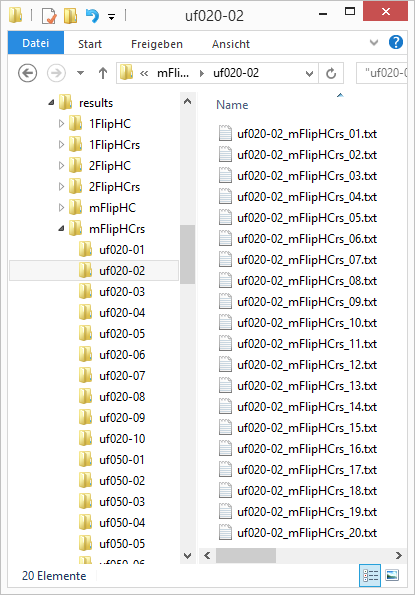
\includegraphics[width=0.33\paperwidth]{graphics/maxsat_example/maxsat_example_log_file_folder_structure}}{0.65}{0.21}%
%
\begin{locateBox}[2-5]{0.65}{0.21}
\begin{pgfpicture}%
\pgfpathrectangle{\pgfpoint{0pt}{0pt}}{\pgfpoint{0.33\paperwidth}{0.79\paperheight}}%
\pgfusepath{use as bounding box,clip}%
%
\pgfsetcolor{alertviolet}%
\pgfsetlinewidth{0.5pt}%
%
\only<3>{%
\pgfpathrectangle{\pgfpoint{0.05\paperwidth}{0.649\paperheight}}{\pgfpoint{0.07\paperwidth}{0.02\paperheight}}%
\pgfpathrectangle{\pgfpoint{0.05\paperwidth}{0.626\paperheight}}{\pgfpoint{0.07\paperwidth}{0.02\paperheight}}%
\pgfpathrectangle{\pgfpoint{0.05\paperwidth}{0.603\paperheight}}{\pgfpoint{0.07\paperwidth}{0.02\paperheight}}%
\pgfpathrectangle{\pgfpoint{0.05\paperwidth}{0.580\paperheight}}{\pgfpoint{0.07\paperwidth}{0.02\paperheight}}%
\pgfpathrectangle{\pgfpoint{0.05\paperwidth}{0.557\paperheight}}{\pgfpoint{0.07\paperwidth}{0.02\paperheight}}%
\pgfpathrectangle{\pgfpoint{0.05\paperwidth}{0.534\paperheight}}{\pgfpoint{0.07\paperwidth}{0.02\paperheight}}%
}%
%
\only<2>{%
\pgfpathrectangle{\pgfpoint{0.272\paperwidth}{0.21\paperheight}}{\pgfpoint{0.018\paperwidth}{0.445\paperheight}}%
\pgfpathrectangle{\pgfpoint{0.013\paperwidth}{0.17\paperheight}}{\pgfpoint{0.06\paperwidth}{0.02\paperheight}}%
}%
%
\only<4>{%
\pgfpathrectangle{\pgfpoint{0.06\paperwidth}{0.319\paperheight}}{\pgfpoint{0.06\paperwidth}{0.212\paperheight}}%
}%
%
\only<5>{%
\pgfpathrectangle{\pgfpoint{0.06\paperwidth}{0.513\paperheight}}{\pgfpoint{0.0433\paperwidth}{0.02\paperheight}}%
\pgfpathrectangle{\pgfpoint{0.06\paperwidth}{0.2958\paperheight}}{\pgfpoint{0.0433\paperwidth}{0.02\paperheight}}%
}%
%
\pgfusepath{stroke}%
%
\end{pgfpicture}%
\end{locateBox}%
\end{frame}%
%
\begin{frame}%
\frametitle{The Flow}%
\begin{itemize}%
\item Having data of this form is a pretty standard situation%
\item<2-> Let us now take a closer look on how the \optimizationBenchmarking\ evaluator is used (and works)%
\end{itemize}%
\locate{}{\pgfuseimage{logo}}{0.725}{0.65}%
\end{frame}%
%
\begin{frame}[b]%
\frametitle{The Flow}%
%
\locate{1-2}{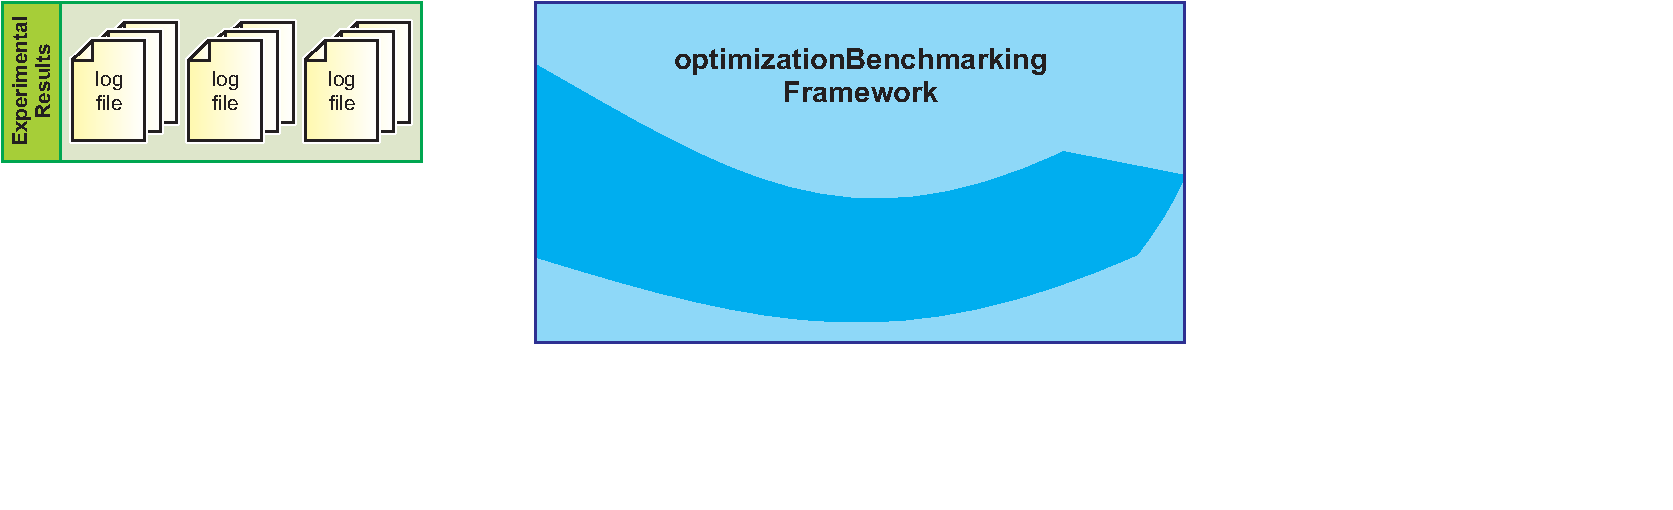
\includegraphics[width=0.9\paperwidth]{graphics/flow/flow_input_1_results}}{0.05}{0.16}%
\locate{3-4}{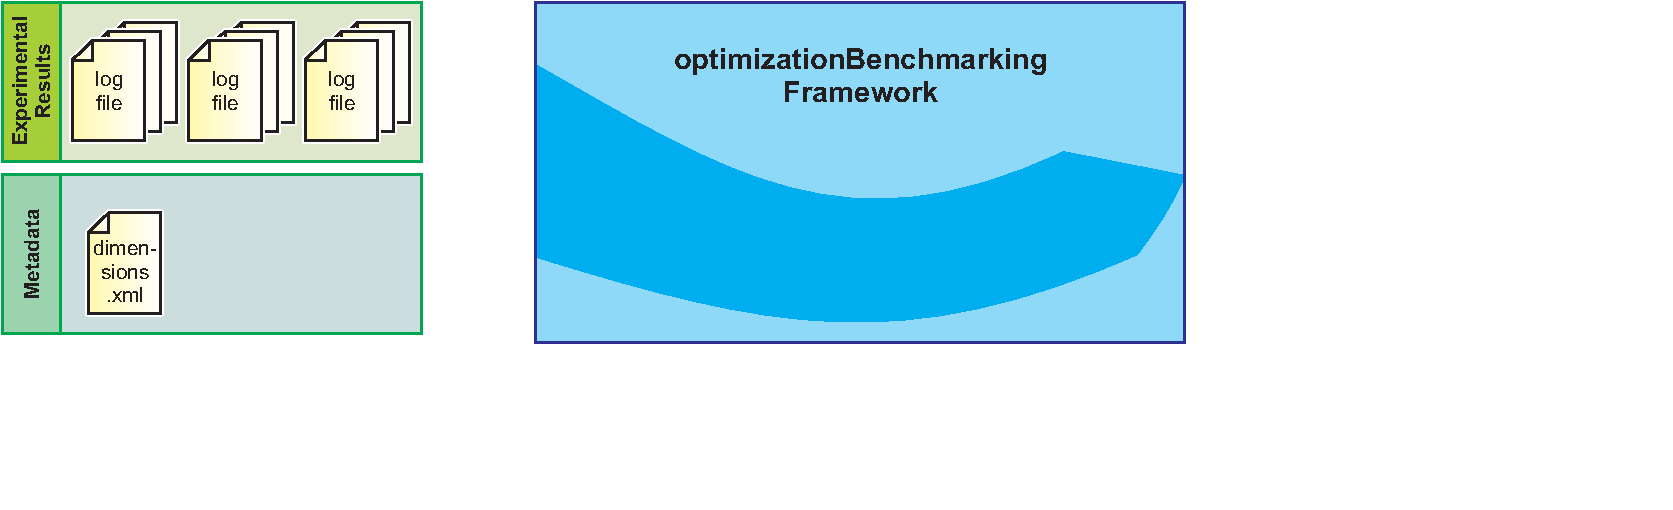
\includegraphics[width=0.9\paperwidth]{graphics/flow/flow_input_2_dimensions}}{0.05}{0.16}%
\locate{5-6}{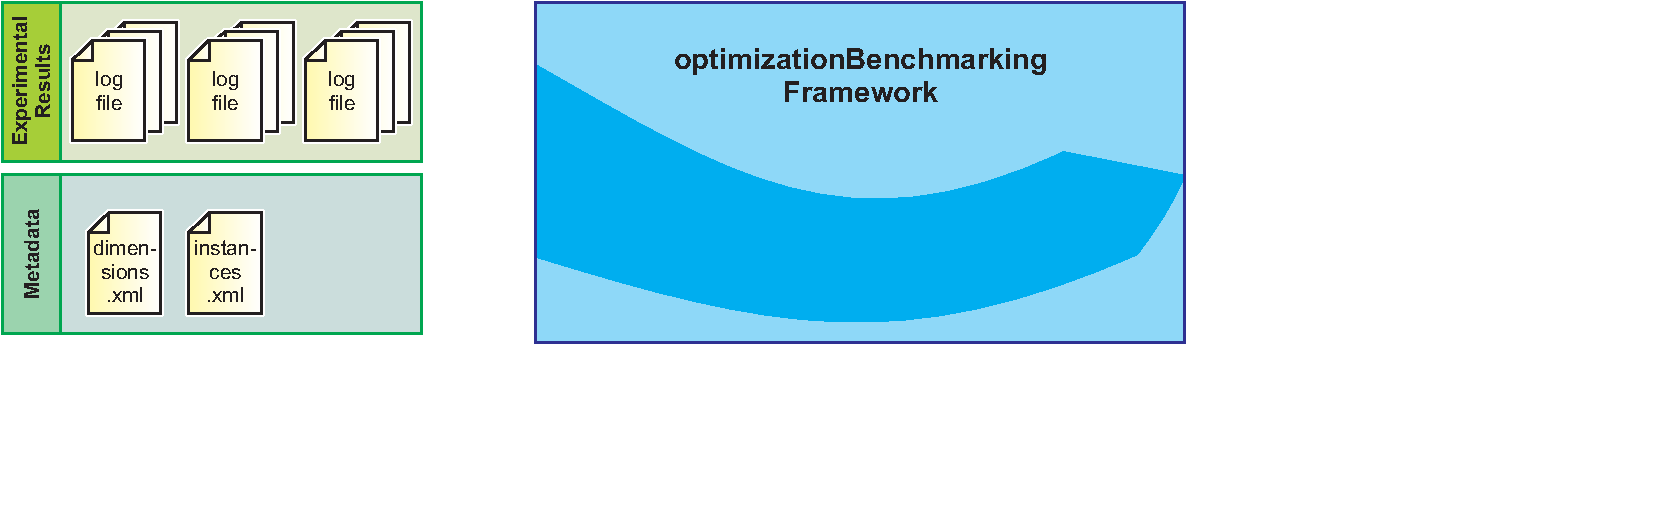
\includegraphics[width=0.9\paperwidth]{graphics/flow/flow_input_3_instances}}{0.05}{0.16}%
\locate{7-8}{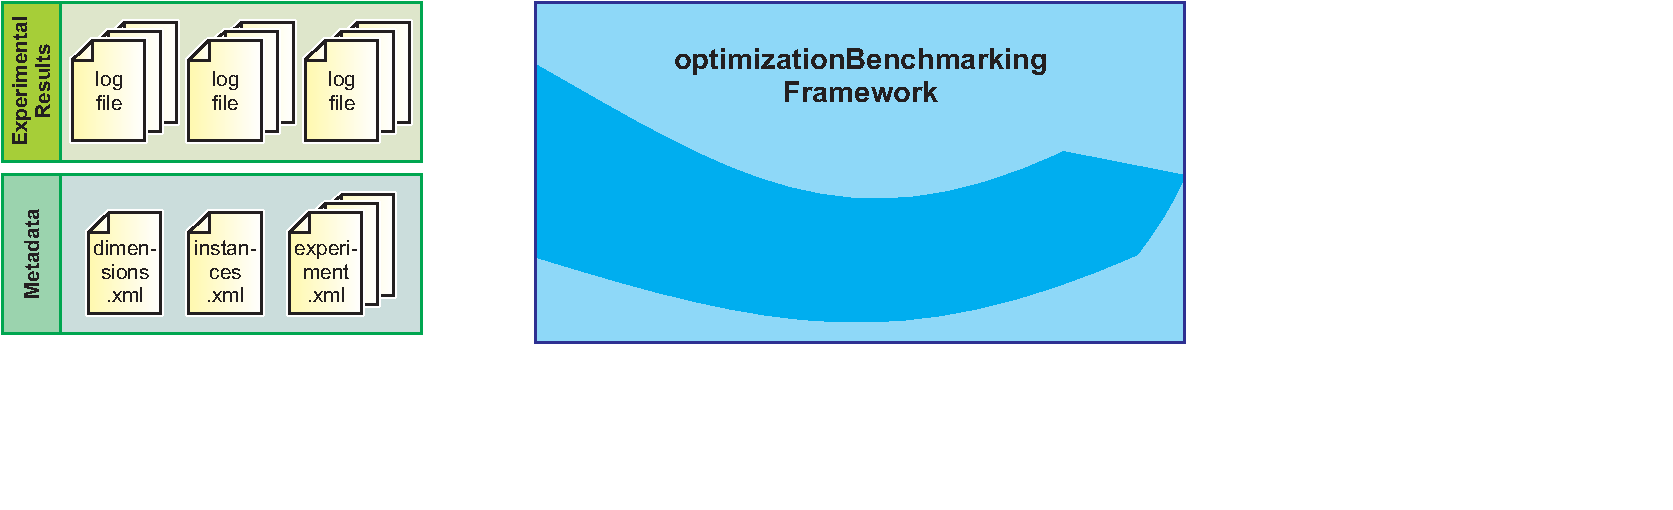
\includegraphics[width=0.9\paperwidth]{graphics/flow/flow_input_4_experiment}}{0.05}{0.16}%
\locate{9-10}{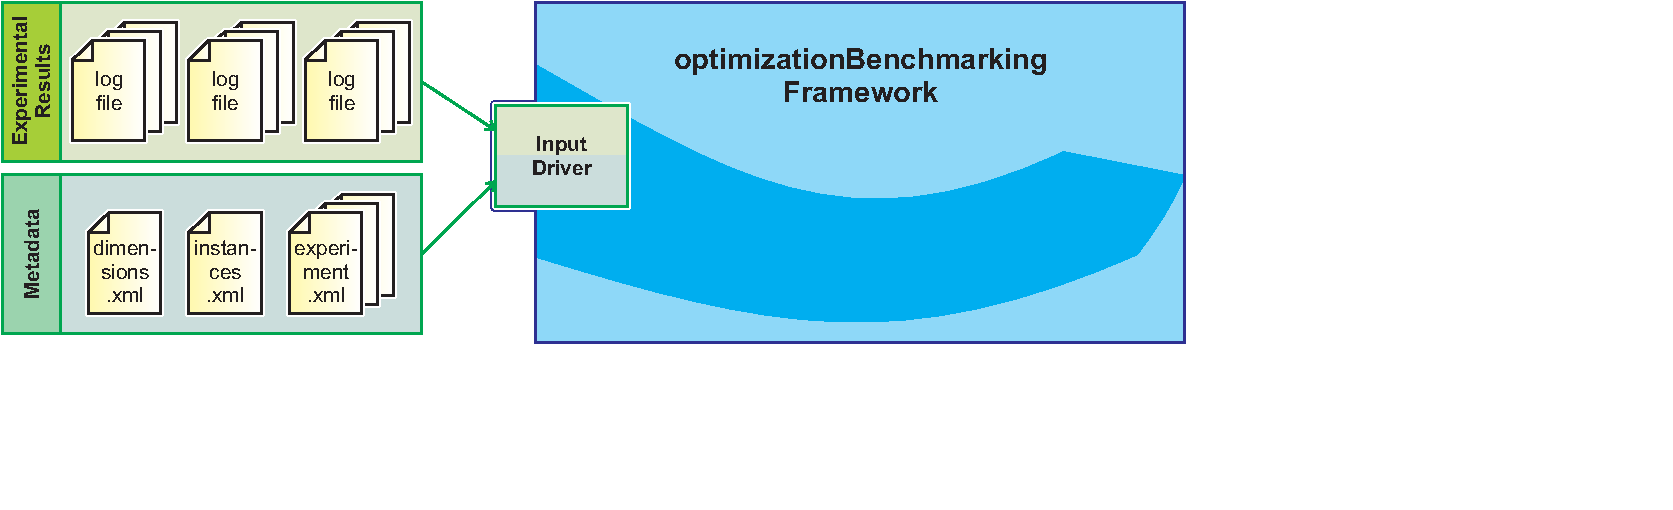
\includegraphics[width=0.9\paperwidth]{graphics/flow/flow_input_5_driver}}{0.05}{0.16}%
\locate{11}{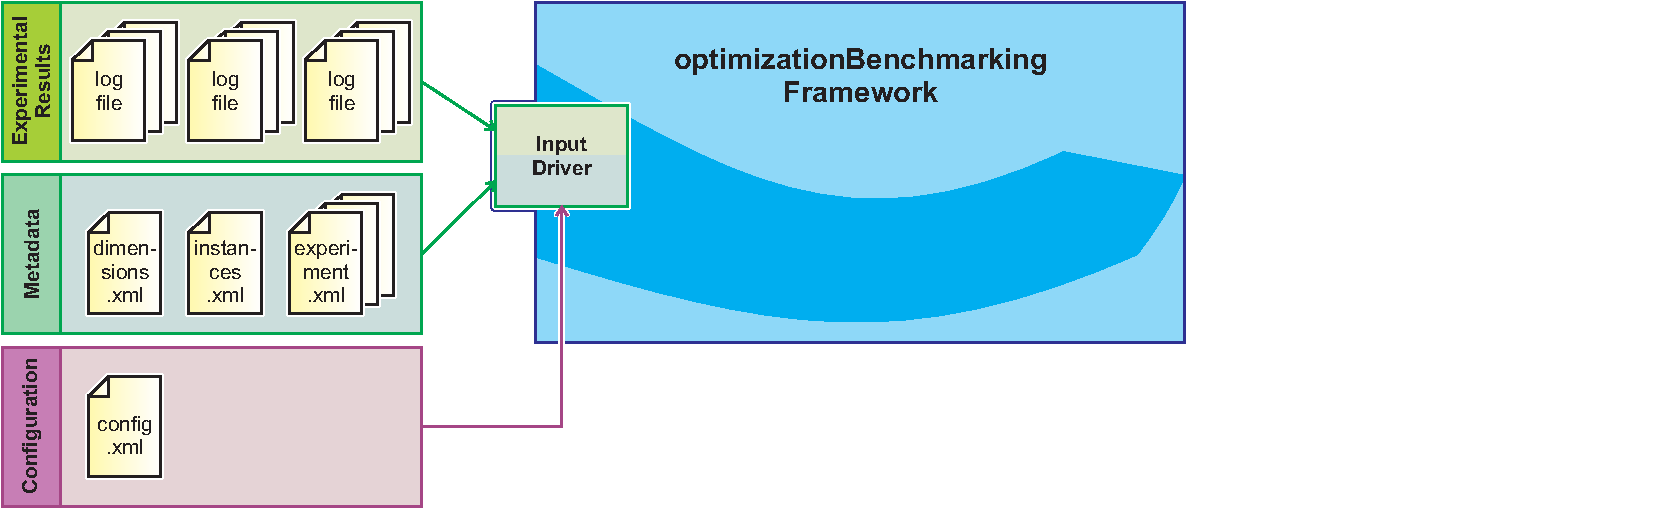
\includegraphics[width=0.9\paperwidth]{graphics/flow/flow_config_1_config}}{0.05}{0.16}%
\locate{12}{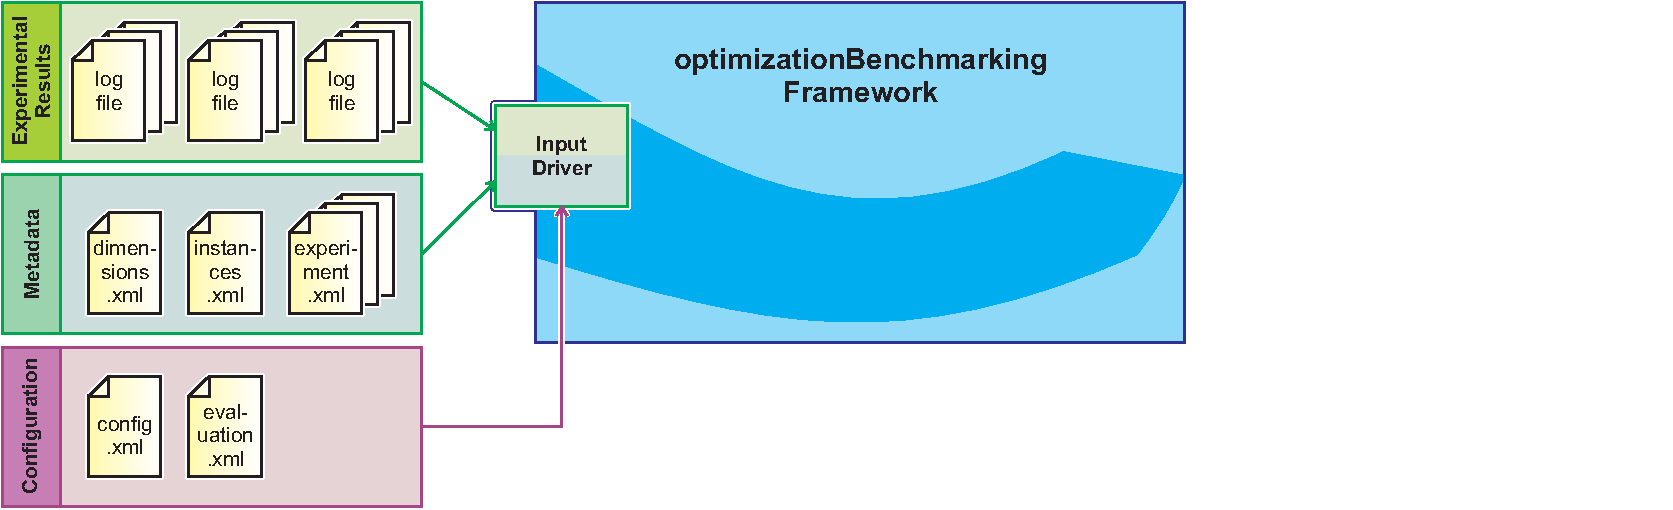
\includegraphics[width=0.9\paperwidth]{graphics/flow/flow_config_2_evaluation}}{0.05}{0.16}%
\locate{13-14}{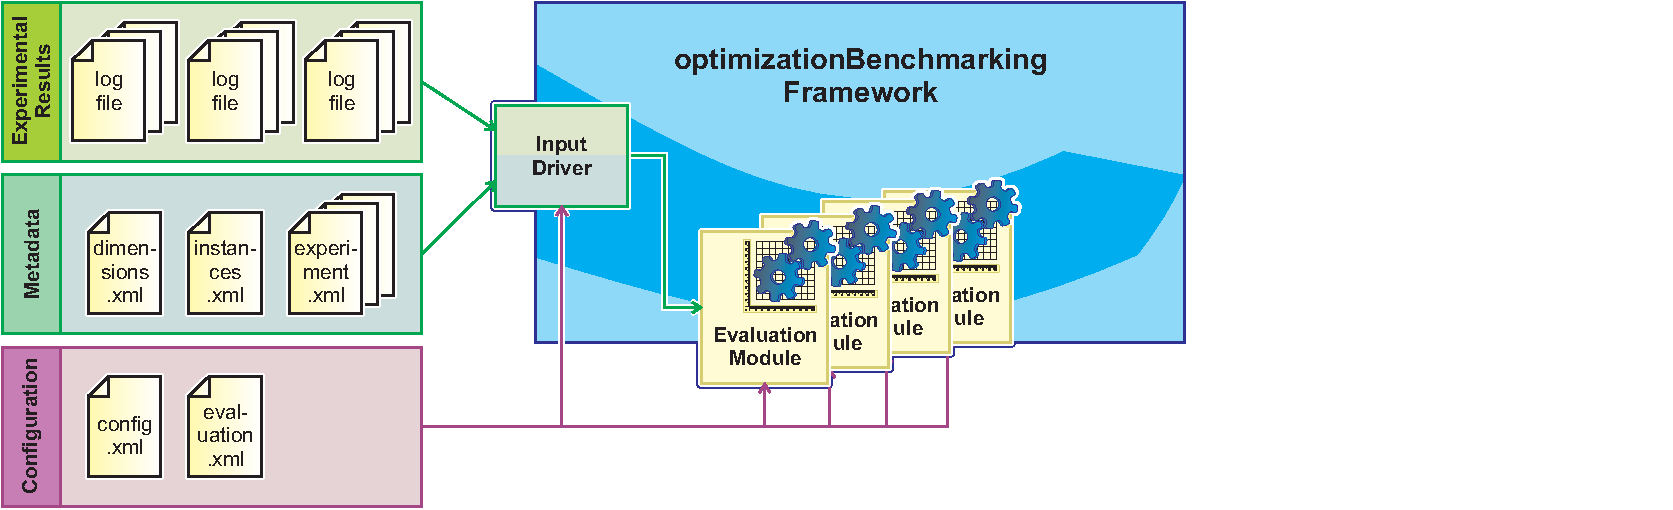
\includegraphics[width=0.9\paperwidth]{graphics/flow/flow_evaluation}}{0.05}{0.16}%
\locate{15}{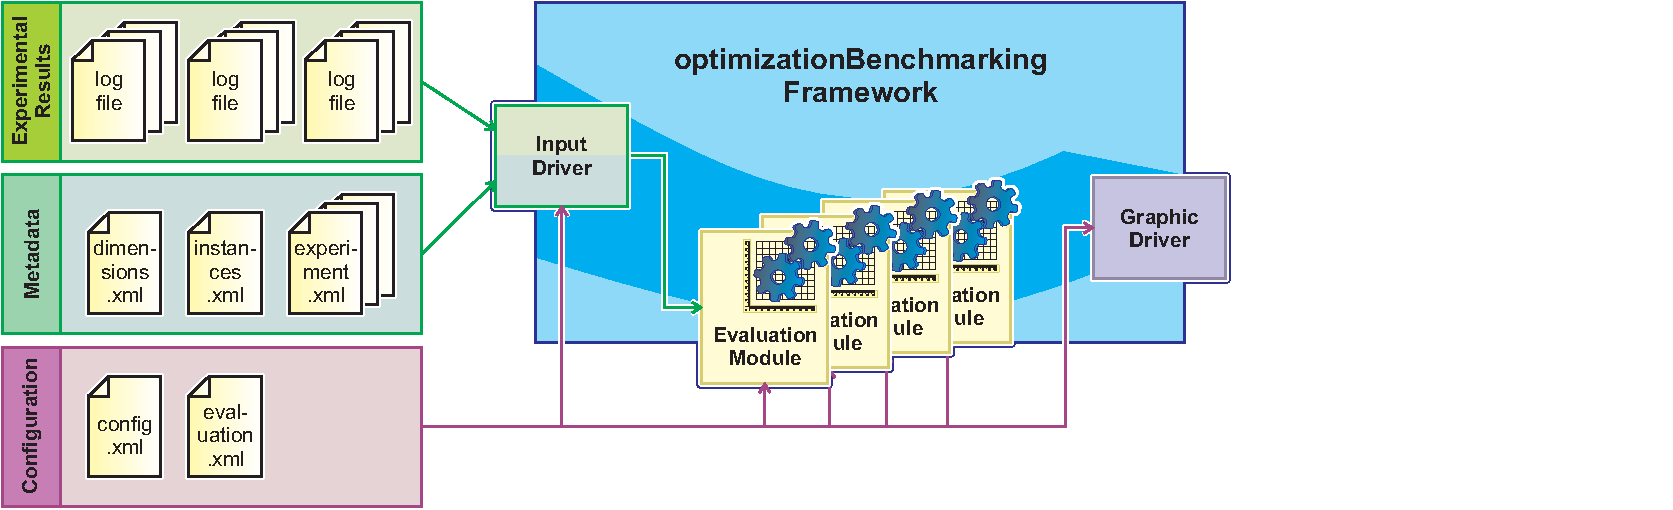
\includegraphics[width=0.9\paperwidth]{graphics/flow/flow_output_1_graphic}}{0.05}{0.16}%
\locate{16}{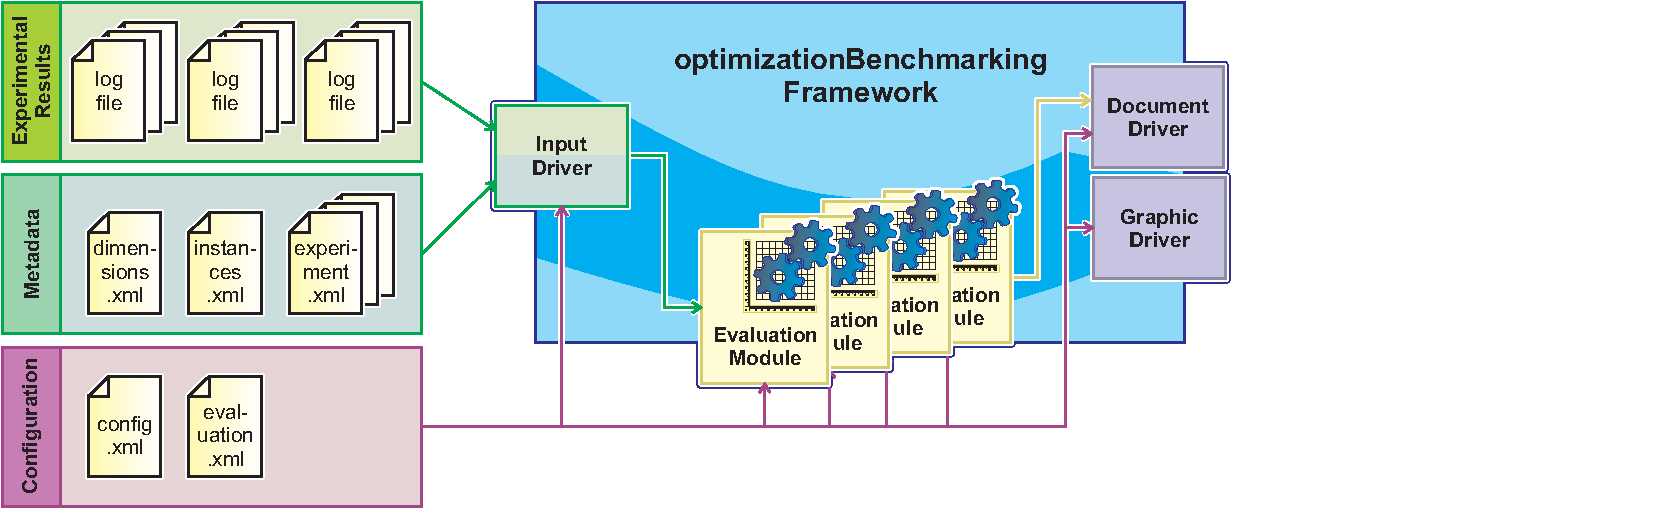
\includegraphics[width=0.9\paperwidth]{graphics/flow/flow_output_2_document}}{0.05}{0.16}%
\locate{17}{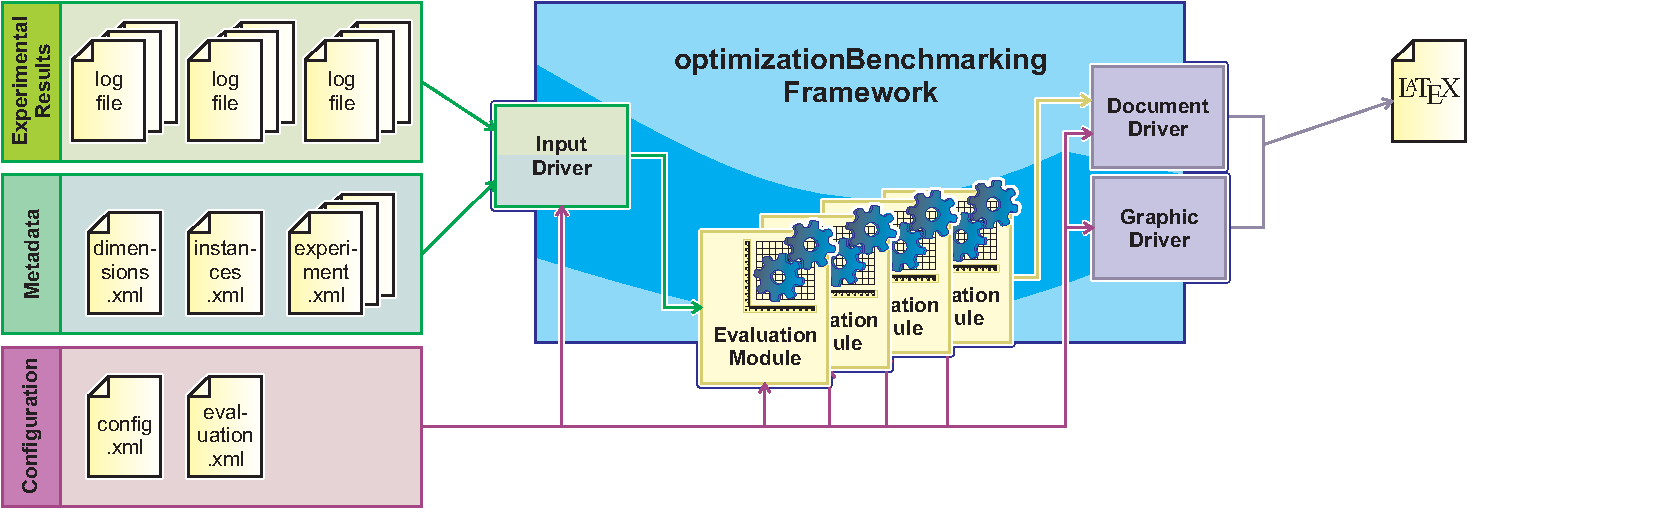
\includegraphics[width=0.9\paperwidth]{graphics/flow/flow_output_3_latex}}{0.05}{0.16}%
\locate{18-20}{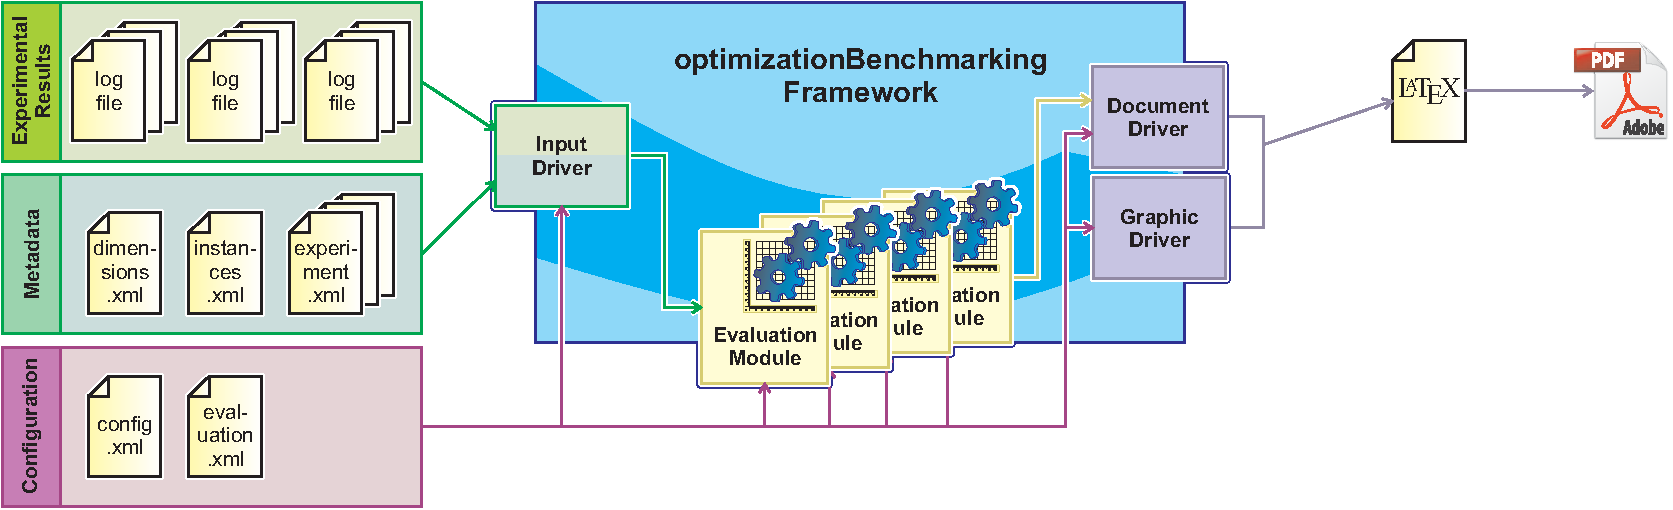
\includegraphics[width=0.9\paperwidth]{graphics/flow/flow_output_4_pdf}}{0.05}{0.16}%
\locate{21}{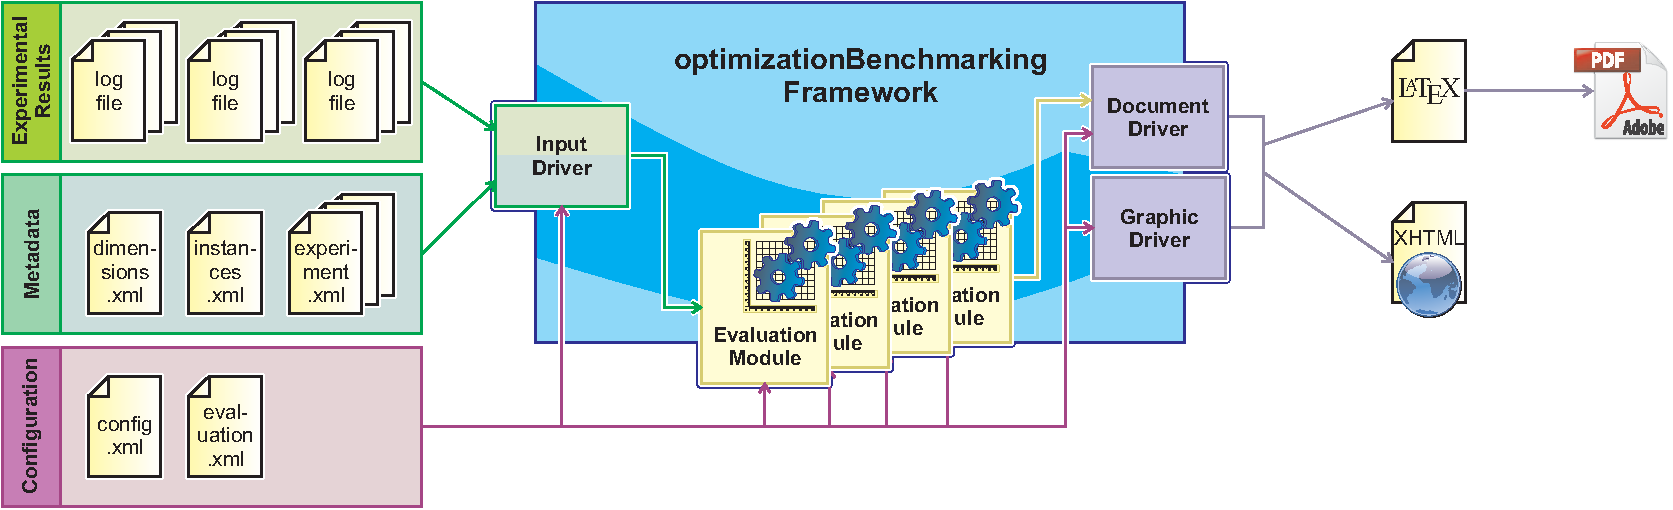
\includegraphics[width=0.9\paperwidth]{graphics/flow/flow_output_5_xhtml}}{0.05}{0.16}%
\locate{22-}{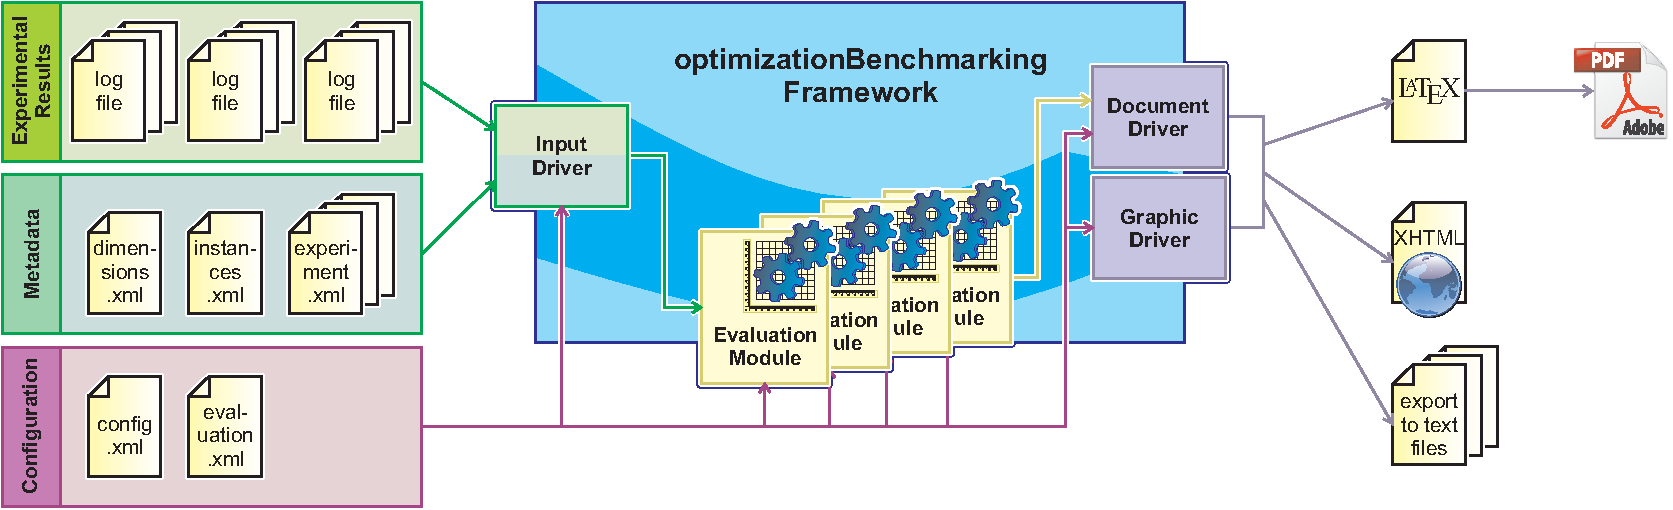
\includegraphics[width=0.9\paperwidth]{graphics/flow/flow}}{0.05}{0.16}%
%
\begin{small}%
\begin{itemize}%
%
\only<-8>{%
\item We got a couple of log files for each experiment\uncover<2->{: 6 experiments in our example, each with $10\times 10\times 20=\numprint{2000}$ log files}%
%}%
%
%\only<3-4>{%
\item<3-> We specify which dimensions we have measured\uncover<4->{: \measureFEs, \measureRuntime, and \measureObjectiveValue\ in our example}%
%}%
%
%\only<5-6>{%
\item<5-> We specify which benchmark instances we have and what their features are\uncover<6->{: $10\times 10$ instances in our example, with features \maxSatVariables\ and \maxSatClauses}%
%}%
%
%\only<7-8>{%
\item<7-> For each experiment, we specify the parameters\uncover<8->{: in our example, these are \texttt{algorithm}, \texttt{operator}, \texttt{restart}}%
}%
%
\only<9-12>{%
\item<9-> An \inQuotes{input driver} loads the data\uncover<10->{: most commonly, the data will be in Comma-, Tab-, or Space-Separated-Values format (\textit{CSV}), but we also support \bbob\expandafter\scitep{\bbobReferences} and \tspSuite\expandafter\scitep{\tspSuiteReferences}}%
%}%
%
%\only<11>{%
\item<11-> Via a configuration file, we choose which input and output formats to use, as well as which file specifies the evaluation process%
%}%
%
%\only<12>{%
\item<12-> The \texttt{evaluation.xml} specifies \emph{how} to evaluate the data, i.e., which evaluation modules to apply%
}%
%
\only<13-14>{%
\item<13-> An evaluation module prints on particular type of information about an experiment or experiment set, such as the ECDF, or a table with final results, etc\dots%
\item<14-> Evaluation modules can be applied multiple times, with different configurations (e.g., we can plot ECDFs for different target solution qualities)%
}%
%
\only<15>{%
\item<15-> We can choose among several different formats to be used for graphics, including EPS\scitep{A1992EPFFS}, PDF\scitep{ISO320002008}, PGF (\LaTeX), SVG(Z), EMF, PNG\scitep{RFC2083}, GIF\scitep{CI1990GIFV8}, BMP, and JPG%
\\\strut%
\vspace{0.18\paperheight}%
\strut\\%
}%
%
%
\only<16-20>{%
\item<16-> We can also choose among different formats for the report documents, including\only<-16>{\dots}%
%
\uncover<17-20>{ %
\LaTeX\scitep{MGBCR2004TLC,GMS1994TLC,L1994LADPSUGARM,OPHS2011TNSSITLOLI1M}\uncover<18->{:%
\begin{itemize}%
\item can automatically be compiled to PDF\scitep{ISO320002008}, if a \LaTeX\ compiler (such as TeXLive\scitep{TEXLIVE} or MiKTeX\scitep{MIKTEX}) is auto-detected%
\item<19-> different document classes, such as IEEEtran\scitep{IEEETRAN}, Springer LLNCS\scitep{SPRINGERLNCS}, ACM sig-alternate\scitep{ACMSIGALTERNATE} can be chosen%
\item<20-> graphic sizes and fonts used in graphics are automatically adapted to document class%
\end{itemize}%
}}%
}%
%
\only<21->{\only<-26>{%
\item<21-> We can also choose among different formats for the report documents, including \LaTeX\only<22->{, }\only<-21>{ and }XHTML\scitep{W3C2010XHTML}%
\only<21>{ for quick viewing in a browser}%
\only<22->{, and a plain text format to export results to other applications}}%
%
\item<23-> Evaluation Modules as well as Input, Document, and Graphic Drivers can easily be added\uncover<24->{: %
implement the corresponding interface%
\uncover<25->{%
, put your class into the classpath%
\uncover<26->{%
, and tell the system to use it in the \texttt{config.xml} or \texttt{evaluation.xml}\dots%
%
\only<27->{%
\item<27-> GUI has simple editors and help for all setup, configuration, and meta-data%
}%
%
}}}%
\only<21>{%
\strut\\\medskip\strut%
}%
\only<22->{%
\strut\medskip\strut%
}%
}%
%
\end{itemize}%
\end{small}%
%
\end{frame}%
%
%
\begin{frame}[t]%
\frametitle{ECDF}%
\begin{itemize}%
\item We can plot the Empirical (Cumulative) Distribution Function (ECDF)\scitep{HAFR2012RPBBOBES,HS1998ELVAPAR,TH2004UAIAEEFSAFSAMS,WCTLTCMY2014BOAAOSFFTTSP} for us, which provides the fraction of runs that have found the solution for their respective problem at a given point in time.%  
\end{itemize}%
%
\locateWithCaption{2-6}{%
\strut\vbox to 0.475\paperheight{\vfil%
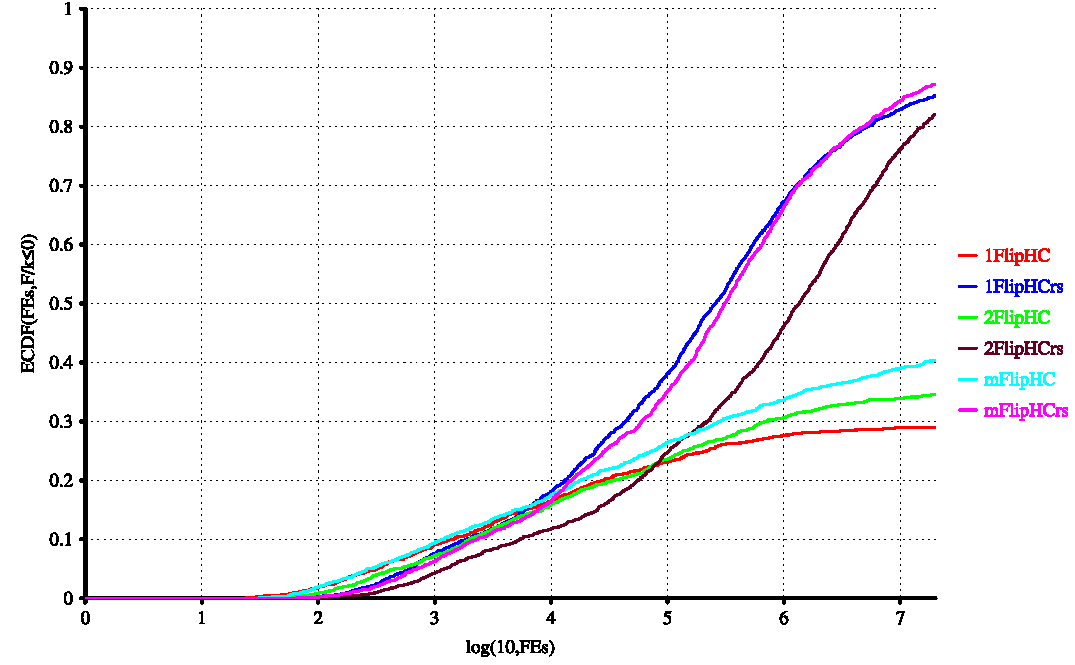
\includegraphics[scale=0.425]{graphics/maxsat_example/ECDF_log_10_FEs_F_k_0/IEEEtran_ECDF_log_10_FEs_F_k_0}%
\strut\hfill\strut%
}%
}{%
The ECDF in over all 100 benchmark instances for time measure \measureFEs\ (log-scaled\only<6->{\alert{, optimized for \texttt{IEEEtran} and two figures per row}}).%
}{0.0375}{0.34}{0.925}%%
%
\locateWithCaption{7}{%
\strut\vbox to 0.475\paperheight{\vfil%
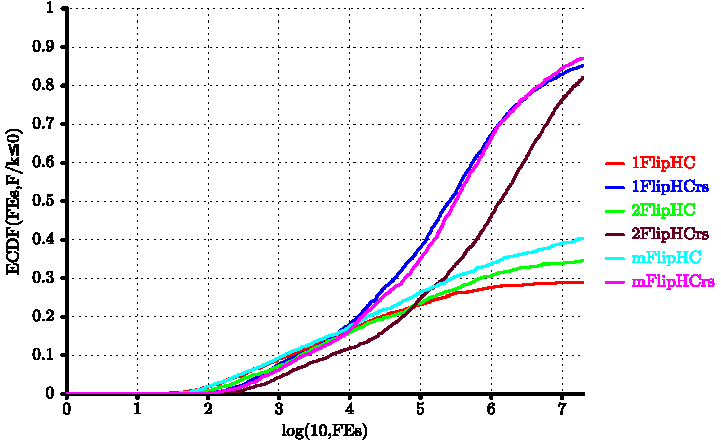
\includegraphics[scale=0.425]{graphics/maxsat_example/ECDF_log_10_FEs_F_k_0/LNCS_ECDF_log_10_FEs_F_k_0}%
\strut\hfill\strut}%
}{%
The ECDF in over all 100 benchmark instances (log-scaled, \alert{optimized for \texttt{LNCS} and two figures per row}).%
}{0.0375}{0.34}{0.925}%
%
\locateWithCaption{8}{%
\strut\vbox to 0.475\paperheight{\vfil%
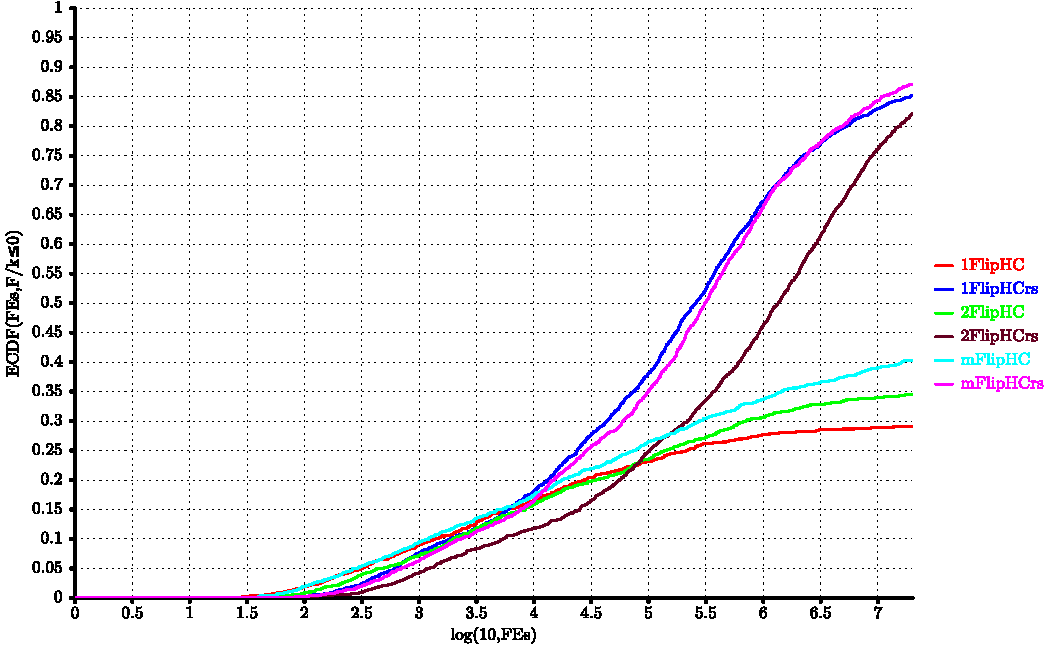
\includegraphics[scale=0.425]{graphics/maxsat_example/ECDF_log_10_FEs_F_k_0/SigAlternate_ECDF_log_10_FEs_F_k_0}%
\strut\hfill\strut}%
}{%
The ECDF in over all 100 benchmark instances (log-scaled, \alert{optimized for \texttt{sig-alternate} and two figures per row}).%
}{0.0375}{0.34}{0.925}%
%
\locateWithCaption{9}{%
\strut\vbox to 0.475\paperheight{\vfil%
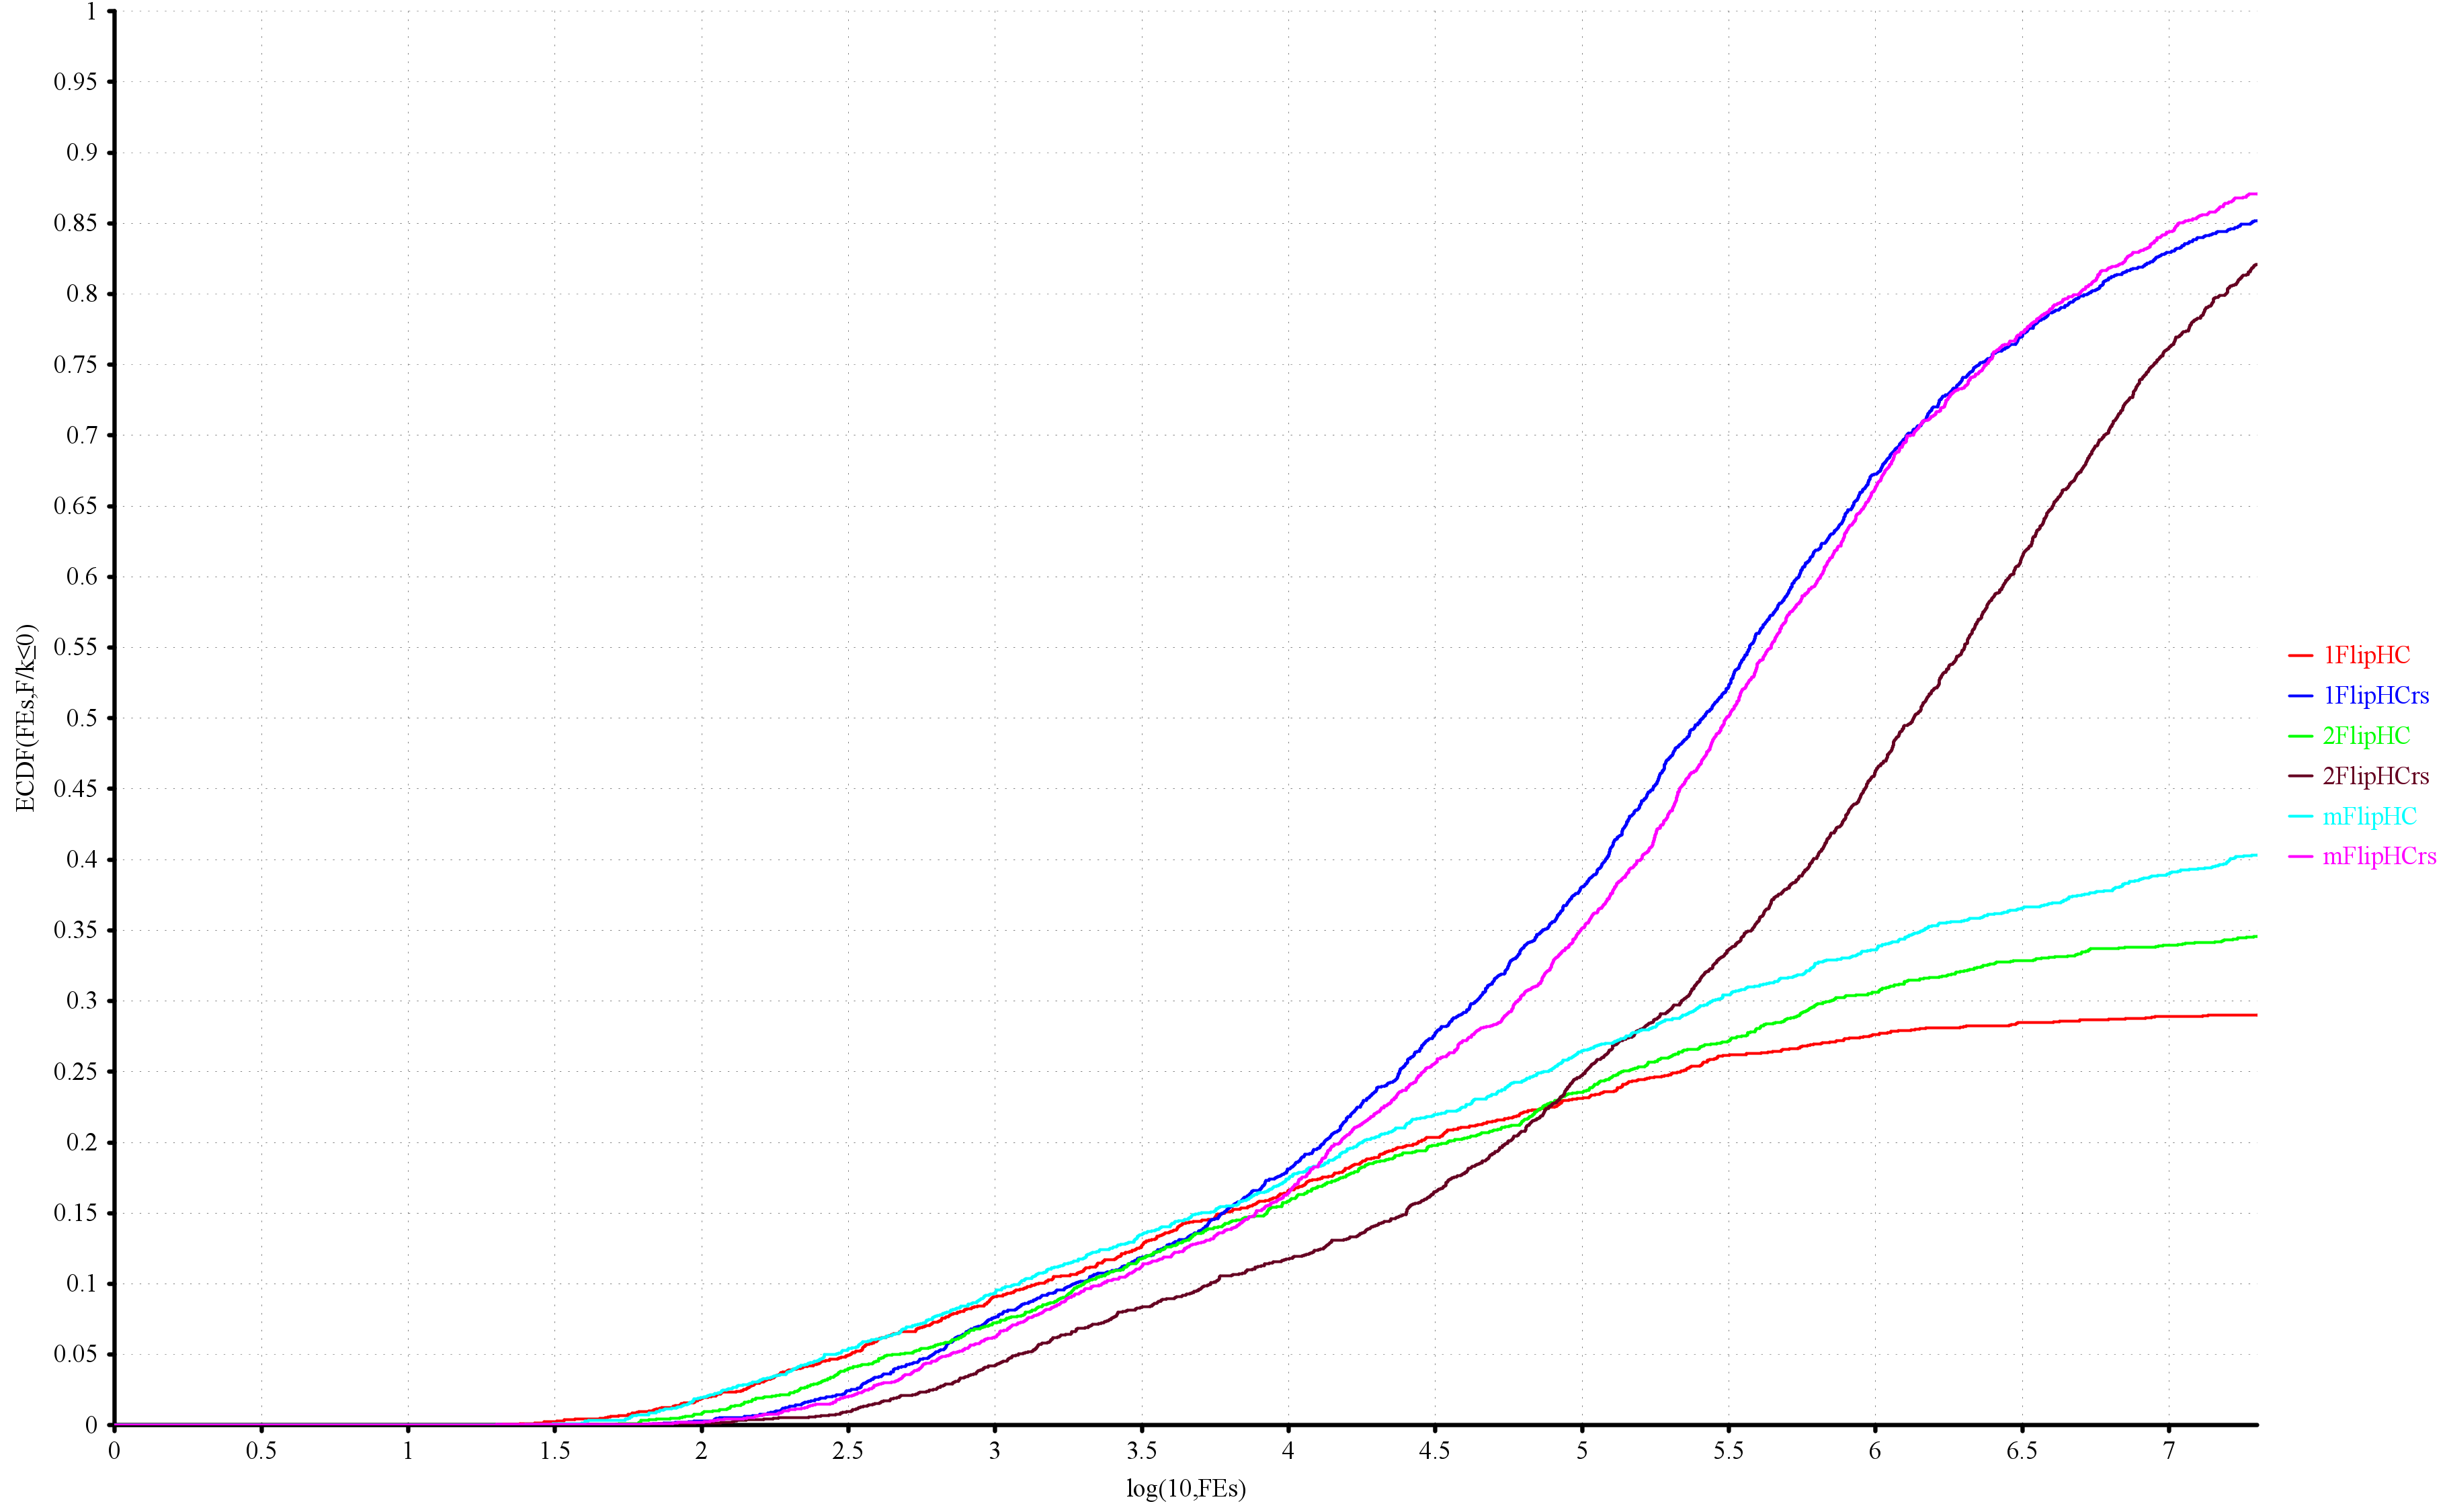
\includegraphics[width=0.6\paperwidth]{graphics/maxsat_example/ECDF_log_10_FEs_F_k_0/XHTML_ECDF_log_10_FEs_F_k_0}%
\strut\hfill\strut}%
}{%
The ECDF in over all 100 benchmark instances (log-scaled, \alert{optimized for \texttt{XHTML} and two figures per row}).%
}{0.0375}{0.34}{0.925}%
%
\locate{3-}{\parbox{0.35\paperwidth}{\small%
\begin{itemize}%
\item the methods with restarts solve more problems (up to 90\%!)%
\item<4-> plain $m$-flips are better than 2-flips are better than 1-flips%
\item<5-> oddly, for restart HCers, there is a tie between the $m$- and 1-flip versions 
\end{itemize}%
}}{0.625}{0.3}%
%
\end{frame}%
%
\begin{frame}%
\frametitle{ECDF for Different Values of \scalebox{1.3}{\ensuremath{\mathbf{\maxSatVariables}}}}%
%
\locate{1-}{%
\parbox{0.234\paperwidth}{\raggedright\small{%
\only<-1>{We now look at the ECDF for different values of \maxSatVariables\ and a goal of 1\% unsatisfied clauses over \measureRuntime\ (log-scaled).}%
\only<2>{For $\maxSatVariables=20$, the methods with restarts are better.}%
\only<3>{But for $\maxSatVariables\geq 50$, those without reach the goal faster.}%
\only<4>{It seems that 1\% unsatisfied clauses can be reached with 1-flips and without restarts.}%
\only<5>{The 2-flip operator again performs worst.}%
\only<6>{It looks as if it gets easier to attain a 1\% error margin if \maxSatVariables\ increases (all ECDFs reach 1).}%
\only<7-8>{For small problems, 1-flip is slightly faster than $m$-flip.}%
\only<9>{For larger problems, $m$-flip becomes slightly faster.}%
\only<10>{All in all, similar behavior over all scales (reaching 1\% error seems to be easy).}%
\only<11->{Only required runtime increases by up to 100 times.}%
}}}{0.013}{0.187}%
%
\locate{1-}{%
\parbox{0.234375\paperwidth}{\centering%
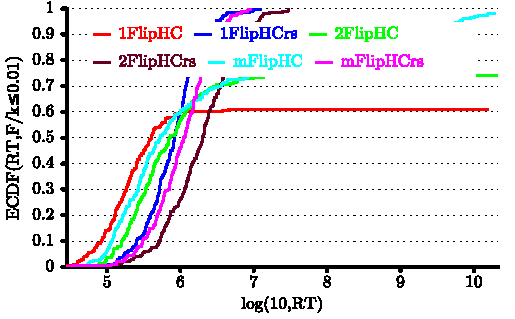
\includegraphics[width=0.234375\paperwidth]{graphics/maxsat_example/ECDF_log_10_RT_F_k_0_01_distinct_n/SigAlternate_ECDF_log_10_RT_F_k_0_01_distinct_n_legend}%
\\\scriptsize{legend}}%
}{0.259375}{0.18}%
%
\locate{2-}{%
\parbox{0.234375\paperwidth}{\centering%
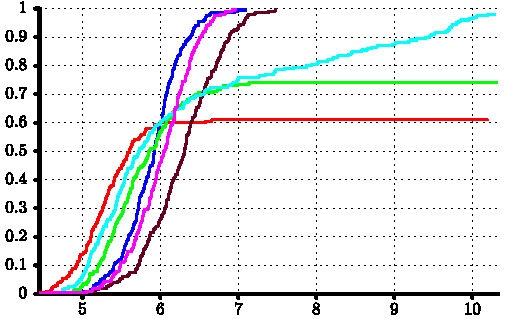
\includegraphics[width=0.234375\paperwidth]{graphics/maxsat_example/ECDF_log_10_RT_F_k_0_01_distinct_n/SigAlternate_ECDF_log_10_RT_F_k_0_01_distinct_n_20}%
\\\scriptsize{$\maxSatVariables=20$}}%
}{0.50625}{0.18}%
%
\locate{3-}{%
\parbox{0.234375\paperwidth}{\centering%
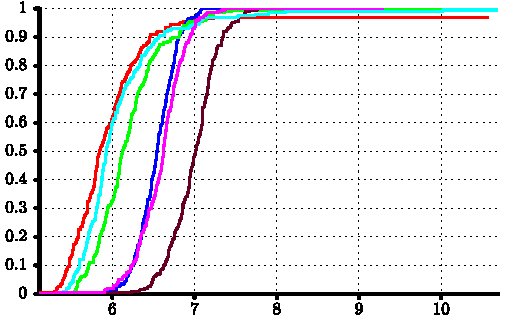
\includegraphics[width=0.234375\paperwidth]{graphics/maxsat_example/ECDF_log_10_RT_F_k_0_01_distinct_n/SigAlternate_ECDF_log_10_RT_F_k_0_01_distinct_n_50}%
\\\scriptsize{$\maxSatVariables=50$}}%
}{0.753125}{0.18}%
%
\locate{4-}{%
\parbox{0.234375\paperwidth}{\centering%
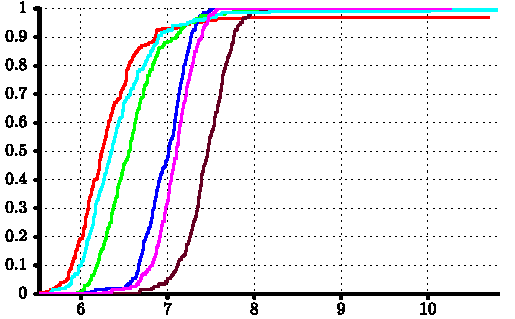
\includegraphics[width=0.234375\paperwidth]{graphics/maxsat_example/ECDF_log_10_RT_F_k_0_01_distinct_n/SigAlternate_ECDF_log_10_RT_F_k_0_01_distinct_n_75}%
\\\scriptsize{$\maxSatVariables=75$}}%
}{0.0125}{0.443333333333333}%
%
\locate{5-}{%
\parbox{0.234375\paperwidth}{\centering%
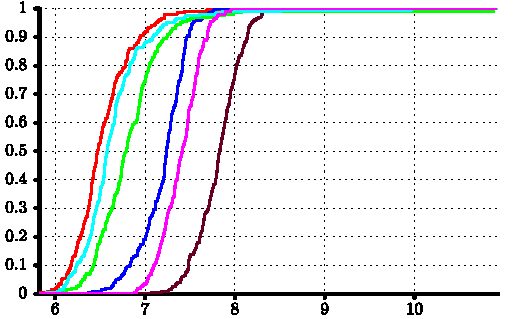
\includegraphics[width=0.234375\paperwidth]{graphics/maxsat_example/ECDF_log_10_RT_F_k_0_01_distinct_n/SigAlternate_ECDF_log_10_RT_F_k_0_01_distinct_n_100}%
\\\scriptsize{$\maxSatVariables=100$}}%
}{0.259375}{0.443333333333333}%
%
\locate{6-}{%
\parbox{0.234375\paperwidth}{\centering%
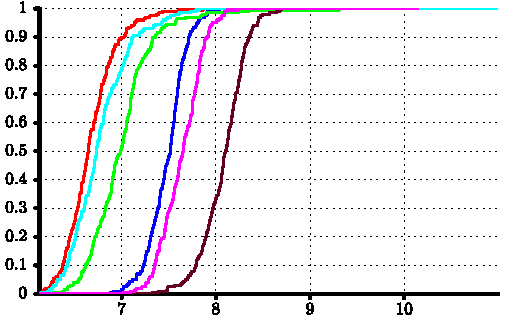
\includegraphics[width=0.234375\paperwidth]{graphics/maxsat_example/ECDF_log_10_RT_F_k_0_01_distinct_n/SigAlternate_ECDF_log_10_RT_F_k_0_01_distinct_n_125}%
\\\scriptsize{$\maxSatVariables=125$}}%
}{0.50625}{0.443333333333333}%
%
\locate{7-}{%
\parbox{0.234375\paperwidth}{\centering%
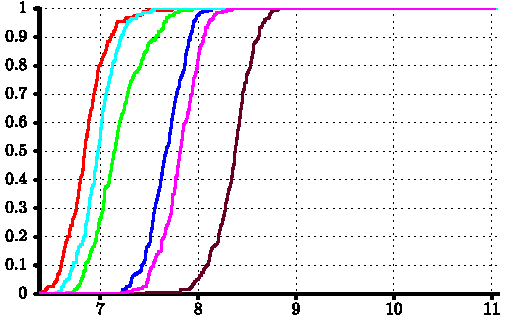
\includegraphics[width=0.234375\paperwidth]{graphics/maxsat_example/ECDF_log_10_RT_F_k_0_01_distinct_n/SigAlternate_ECDF_log_10_RT_F_k_0_01_distinct_n_150}%
\\\scriptsize{$\maxSatVariables=150$}}%
}{0.753125}{0.443333333333333}%
%
\locate{8-}{%
\parbox{0.234375\paperwidth}{\centering%
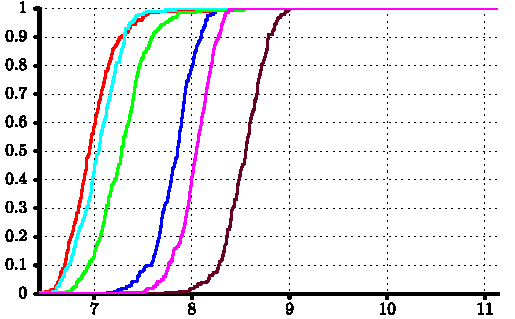
\includegraphics[width=0.234375\paperwidth]{graphics/maxsat_example/ECDF_log_10_RT_F_k_0_01_distinct_n/SigAlternate_ECDF_log_10_RT_F_k_0_01_distinct_n_175}%
\\\scriptsize{$\maxSatVariables=175$}}%
}{0.0125}{0.706666666666667}%
%
\locate{9-}{%
\parbox{0.234375\paperwidth}{\centering%
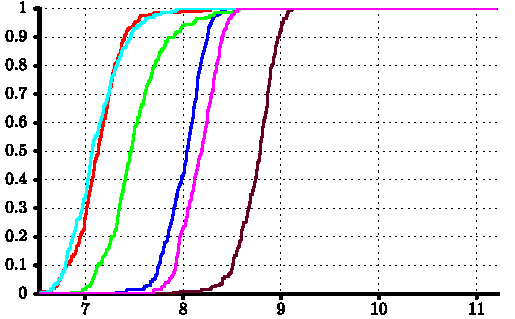
\includegraphics[width=0.234375\paperwidth]{graphics/maxsat_example/ECDF_log_10_RT_F_k_0_01_distinct_n/SigAlternate_ECDF_log_10_RT_F_k_0_01_distinct_n_200}%
\\\scriptsize{$\maxSatVariables=200$}}%
}{0.259375}{0.706666666666667}%%
%
\locate{10-}{%
\parbox{0.234375\paperwidth}{\centering%
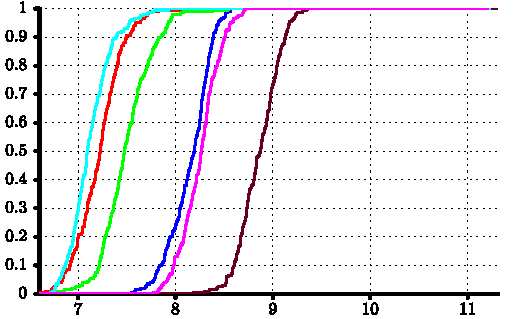
\includegraphics[width=0.234375\paperwidth]{graphics/maxsat_example/ECDF_log_10_RT_F_k_0_01_distinct_n/SigAlternate_ECDF_log_10_RT_F_k_0_01_distinct_n_225}%
\\\scriptsize{$\maxSatVariables=225$}}%
}{0.50625}{0.706666666666667}%
%
\locate{11-}{%
\parbox{0.234375\paperwidth}{\centering%
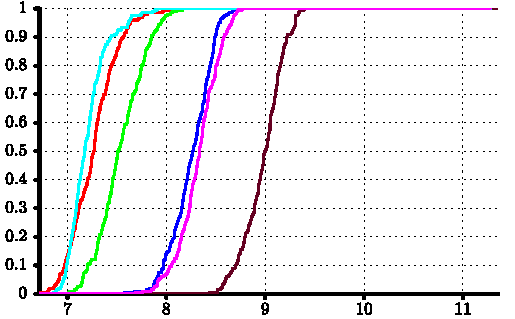
\includegraphics[width=0.234375\paperwidth]{graphics/maxsat_example/ECDF_log_10_RT_F_k_0_01_distinct_n/SigAlternate_ECDF_log_10_RT_F_k_0_01_distinct_n_250}%
\\\scriptsize{$\maxSatVariables=250$}}%
}{0.753125}{0.706666666666667}%
%
\end{frame}%
%
%
\begin{frame}%
\frametitle{Progress for Different Values of \scalebox{1.3}{\ensuremath{\mathbf{\maxSatClauses}}}}%
%
\locate{1-}{%
\parbox{0.234\paperwidth}{\raggedright\small{%
\only<-1>{We now look at the progress curves (\measureObjectiveValue\ over \measureFEs\ divided by\footnote<1>{We normalize \measureFEs\ with \maxSatVariables\ in the hope to make the time measure comparable over different \maxSatVariables.} \maxSatVariables, log-scaled) for different values of \maxSatClauses.}%
\only<2>{For very small-scale problems, all algorithms behave similar.}%
\only<3>{But soon, two groups form: with and without restarts.}%
\only<4>{Algorithms using \emph{my example restart policy} seem to be slower.}%
\only<5>{The gap increases with rising \maxSatClauses}%
\only<6>{Thus, we find: algorithms with my restart policy are slower than those without\dots}%
\only<7>{{\dots}but from the ECDF we know they can solve more problems eventually.}%
\only<8>{For all scales, the initial random solutions, seem to have about 12\% of unsatisfied clauses (in median).}%
\only<9->{Convergence seems to happen between 100\maxSatVariables\ and 1000\maxSatVariables}%
}}}{0.013}{0.187}%
%
\locate{1-}{%
\parbox{0.234375\paperwidth}{\centering%
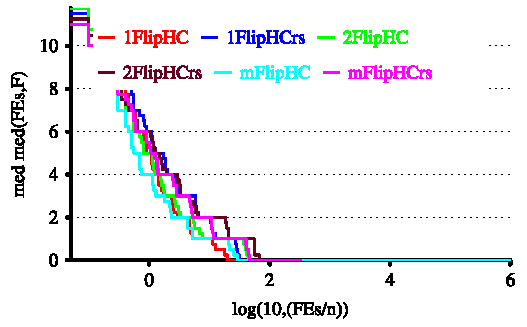
\includegraphics[width=0.234375\paperwidth]{graphics/maxsat_example/med_med_log_10_FEs_n_F_distinct_k/IEEEtran_med_med_log_10_FEs_n_F_distinct_k_legend}%
\\\scriptsize{legend}}%
}{0.259375}{0.18}%
%
\locate{2-}{%
\parbox{0.234375\paperwidth}{\centering%
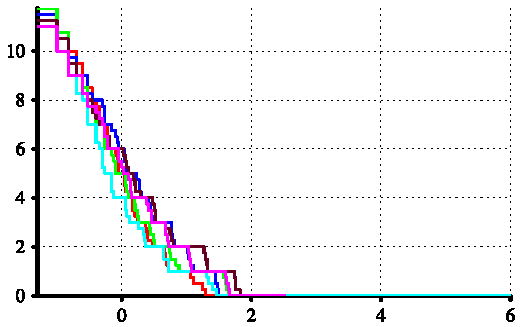
\includegraphics[width=0.234375\paperwidth]{graphics/maxsat_example/med_med_log_10_FEs_n_F_distinct_k/IEEEtran_med_med_log_10_FEs_n_F_distinct_k_91}%
\\\scriptsize{$\maxSatClauses=91$}}%
}{0.50625}{0.18}%
%
\locate{3-}{%
\parbox{0.234375\paperwidth}{\centering%
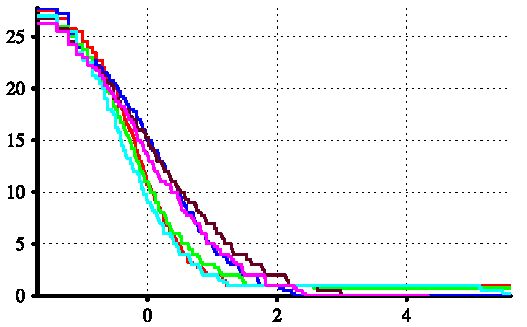
\includegraphics[width=0.234375\paperwidth]{graphics/maxsat_example/med_med_log_10_FEs_n_F_distinct_k/IEEEtran_med_med_log_10_FEs_n_F_distinct_k_218}%
\\\scriptsize{$\maxSatClauses=218$}}%
}{0.753125}{0.18}%
%
\locate{4-}{%
\parbox{0.234375\paperwidth}{\centering%
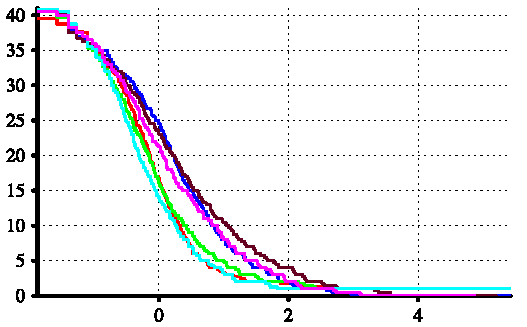
\includegraphics[width=0.234375\paperwidth]{graphics/maxsat_example/med_med_log_10_FEs_n_F_distinct_k/IEEEtran_med_med_log_10_FEs_n_F_distinct_k_325}%
\\\scriptsize{$\maxSatClauses=325$}}%
}{0.0125}{0.443333333333333}%
%
\locate{5-}{%
\parbox{0.234375\paperwidth}{\centering%
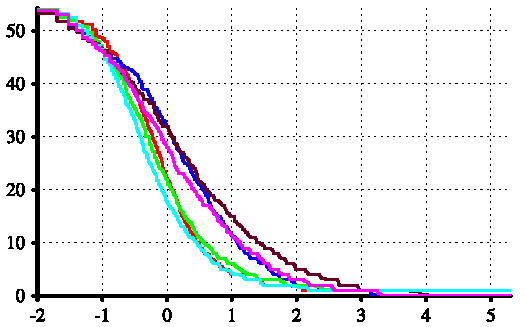
\includegraphics[width=0.234375\paperwidth]{graphics/maxsat_example/med_med_log_10_FEs_n_F_distinct_k/IEEEtran_med_med_log_10_FEs_n_F_distinct_k_430}%
\\\scriptsize{$\maxSatClauses=430$}}%
}{0.259375}{0.443333333333333}%
%
\locate{6-}{%
\parbox{0.234375\paperwidth}{\centering%
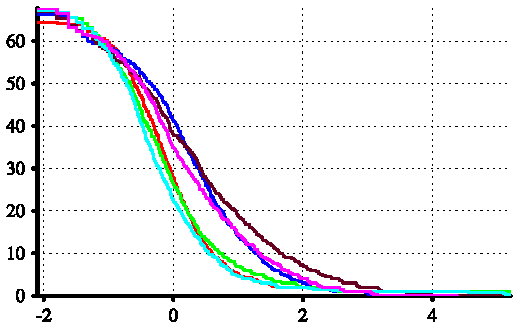
\includegraphics[width=0.234375\paperwidth]{graphics/maxsat_example/med_med_log_10_FEs_n_F_distinct_k/IEEEtran_med_med_log_10_FEs_n_F_distinct_k_538}%
\\\scriptsize{$\maxSatClauses=538$}}%
}{0.50625}{0.443333333333333}%
%
\locate{7-}{%
\parbox{0.234375\paperwidth}{\centering%
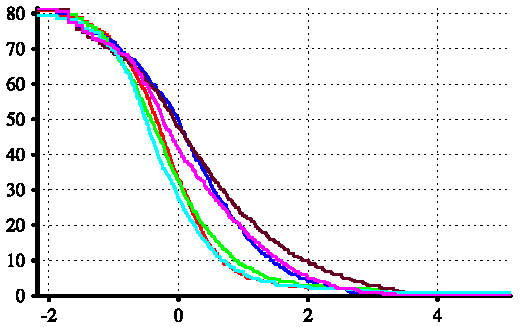
\includegraphics[width=0.234375\paperwidth]{graphics/maxsat_example/med_med_log_10_FEs_n_F_distinct_k/IEEEtran_med_med_log_10_FEs_n_F_distinct_k_645}%
\\\scriptsize{$\maxSatClauses=645$}}%
}{0.753125}{0.443333333333333}%
%
\locate{8-}{%
\parbox{0.234375\paperwidth}{\centering%
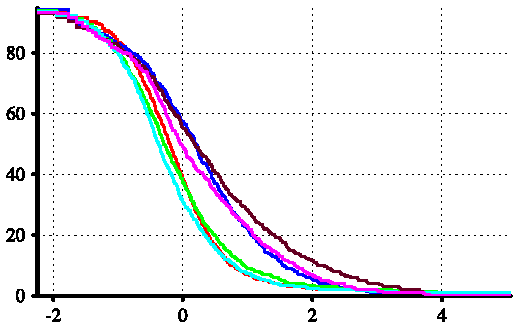
\includegraphics[width=0.234375\paperwidth]{graphics/maxsat_example/med_med_log_10_FEs_n_F_distinct_k/IEEEtran_med_med_log_10_FEs_n_F_distinct_k_753}%
\\\scriptsize{$\maxSatClauses=753$}}%
}{0.0125}{0.706666666666667}%
%
\locate{9-}{%
\parbox{0.234375\paperwidth}{\centering%
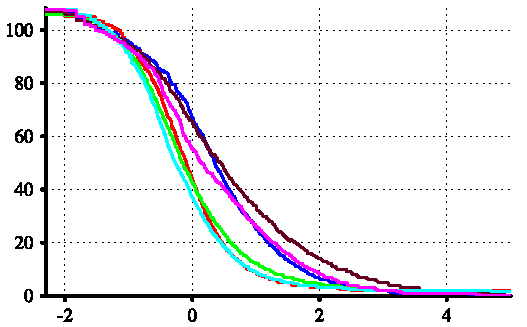
\includegraphics[width=0.234375\paperwidth]{graphics/maxsat_example/med_med_log_10_FEs_n_F_distinct_k/IEEEtran_med_med_log_10_FEs_n_F_distinct_k_860}%
\\\scriptsize{$\maxSatClauses=860$}}%
}{0.259375}{0.706666666666667}%%
%
\locate{10-}{%
\parbox{0.234375\paperwidth}{\centering%
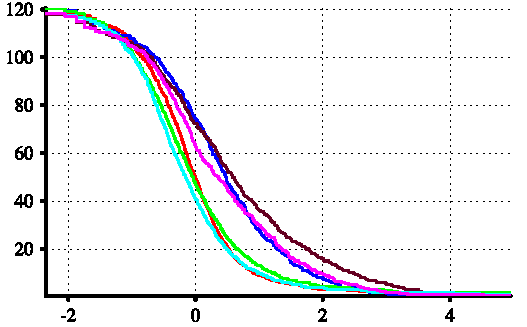
\includegraphics[width=0.234375\paperwidth]{graphics/maxsat_example/med_med_log_10_FEs_n_F_distinct_k/IEEEtran_med_med_log_10_FEs_n_F_distinct_k_960}%
\\\scriptsize{$\maxSatClauses=960$}}%
}{0.50625}{0.706666666666667}%
%
\locate{11-}{%
\parbox{0.234375\paperwidth}{\centering%
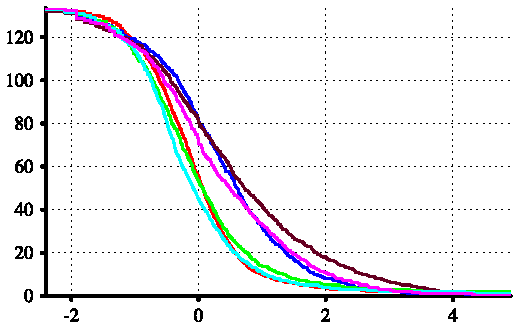
\includegraphics[width=0.234375\paperwidth]{graphics/maxsat_example/med_med_log_10_FEs_n_F_distinct_k/IEEEtran_med_med_log_10_FEs_n_F_distinct_k_1065}%
\\\scriptsize{$\maxSatClauses=1065$}}%
}{0.753125}{0.706666666666667}%
%
\end{frame}%
%
%
\begin{frame}%
\frametitle{StdDev of \measureObjectiveValue\ for Different Values of \scalebox{1.3}{\ensuremath{\mathbf{\maxSatVariables}}}}%
%
\locate{1-}{%
\parbox{0.234\paperwidth}{\raggedright\small{%
\only<-1>{Let's look at the standard deviation of the best objective value \measureObjectiveValue\ (divided by\footnote<1>{Since \measureObjectiveValue\ is always in $1\dots\maxSatClauses$, dividing it by \maxSatClauses\ normalizes it into $[0,1]$ and makes the values comparable for different \maxSatClauses\ or \maxSatVariables.} \maxSatClauses) found over \measureRuntime\ (log-scaled) for different values of \maxSatVariables.}%
\only<2>{For small-scale problems, the standard deviation seems to decrease steadily.}%
\only<3>{The reason is probably that the algorithms converge nicely.}%
\only<4>{For the methods with restarts, it reaches very close to 0.}%
\only<5>{For those without, it remains constant above 0 after some time.}%
\only<6>{These algorithms probably get stuck at different local optima in different runs.}%
\only<7>{For increasing scales, the standard deviation goes first down, then up, then farther down.}%
\only<8>{Maybe there is some kind of hard-to-attain improvement that some runs find earlier than others.}%
\only<9>{The time of convergence seems to increase for the methods with restarts with \maxSatVariables.}%
\only<10->{The early standard deviations are usually below 0.03 and highest for small \maxSatVariables.}% 
}}}{0.013}{0.187}%
%
\locate{1-}{%
\parbox{0.234375\paperwidth}{\centering%
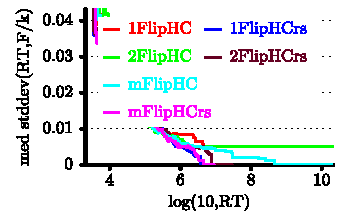
\includegraphics[width=0.234375\paperwidth]{graphics/maxsat_example/med_stddev_log_10_RT_F_k_distinct_n/LNCS_med_stddev_log_10_RT_F_k_distinct_n_legend}%
\\\scriptsize{legend}}%
}{0.259375}{0.18}%
%
\locate{2-}{%
\parbox{0.234375\paperwidth}{\centering%
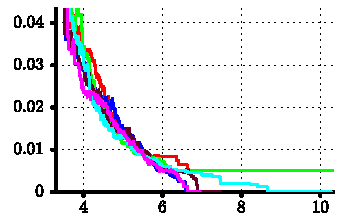
\includegraphics[width=0.234375\paperwidth]{graphics/maxsat_example/med_stddev_log_10_RT_F_k_distinct_n/LNCS_med_stddev_log_10_RT_F_k_distinct_n_20}%
\\\scriptsize{$\maxSatVariables=20$}}%
}{0.50625}{0.18}%
%
\locate{3-}{%
\parbox{0.234375\paperwidth}{\centering%
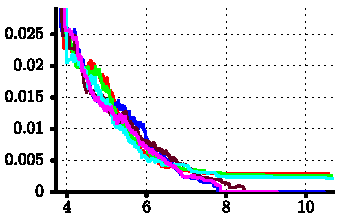
\includegraphics[width=0.234375\paperwidth]{graphics/maxsat_example/med_stddev_log_10_RT_F_k_distinct_n/LNCS_med_stddev_log_10_RT_F_k_distinct_n_50}%
\\\scriptsize{$\maxSatVariables=50$}}%
}{0.753125}{0.18}%
%
\locate{4-}{%
\parbox{0.234375\paperwidth}{\centering%
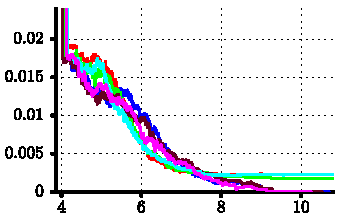
\includegraphics[width=0.234375\paperwidth]{graphics/maxsat_example/med_stddev_log_10_RT_F_k_distinct_n/LNCS_med_stddev_log_10_RT_F_k_distinct_n_75}%
\\\scriptsize{$\maxSatVariables=75$}}%
}{0.0125}{0.443333333333333}%
%
\locate{5-}{%
\parbox{0.234375\paperwidth}{\centering%
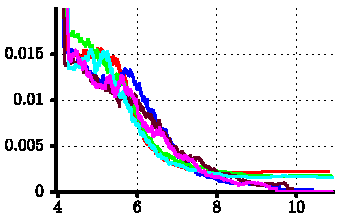
\includegraphics[width=0.234375\paperwidth]{graphics/maxsat_example/med_stddev_log_10_RT_F_k_distinct_n/LNCS_med_stddev_log_10_RT_F_k_distinct_n_100}%
\\\scriptsize{$\maxSatVariables=100$}}%
}{0.259375}{0.443333333333333}%
%
\locate{6-}{%
\parbox{0.234375\paperwidth}{\centering%
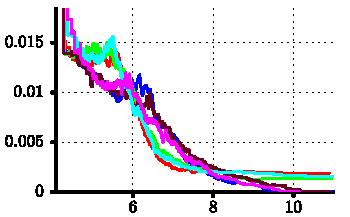
\includegraphics[width=0.234375\paperwidth]{graphics/maxsat_example/med_stddev_log_10_RT_F_k_distinct_n/LNCS_med_stddev_log_10_RT_F_k_distinct_n_125}%
\\\scriptsize{$\maxSatVariables=125$}}%
}{0.50625}{0.443333333333333}%
%
\locate{7-}{%
\parbox{0.234375\paperwidth}{\centering%
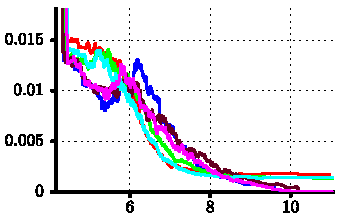
\includegraphics[width=0.234375\paperwidth]{graphics/maxsat_example/med_stddev_log_10_RT_F_k_distinct_n/LNCS_med_stddev_log_10_RT_F_k_distinct_n_150}%
\\\scriptsize{$\maxSatVariables=150$}}%
}{0.753125}{0.443333333333333}%
%
\locate{8-}{%
\parbox{0.234375\paperwidth}{\centering%
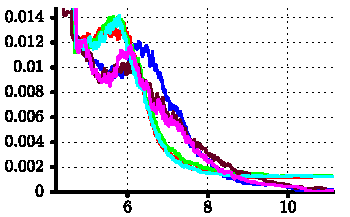
\includegraphics[width=0.234375\paperwidth]{graphics/maxsat_example/med_stddev_log_10_RT_F_k_distinct_n/LNCS_med_stddev_log_10_RT_F_k_distinct_n_175}%
\\\scriptsize{$\maxSatVariables=175$}}%
}{0.0125}{0.706666666666667}%
%
\locate{9-}{%
\parbox{0.234375\paperwidth}{\centering%
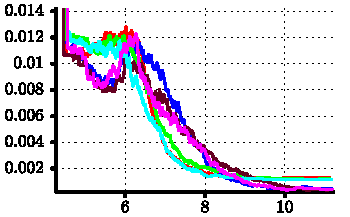
\includegraphics[width=0.234375\paperwidth]{graphics/maxsat_example/med_stddev_log_10_RT_F_k_distinct_n/LNCS_med_stddev_log_10_RT_F_k_distinct_n_200}%
\\\scriptsize{$\maxSatVariables=200$}}%
}{0.259375}{0.706666666666667}%%
%
\locate{10-}{%
\parbox{0.234375\paperwidth}{\centering%
\includegraphics[width=0.234375\paperwidth]{graphics/maxsat_example/med_stddev_log_10_RT_F_k_distinct_n/LNCS_med_stddev_log_10_RT_F_k_distinct_n_225}%
\\\scriptsize{$\maxSatVariables=225$}}%
}{0.50625}{0.706666666666667}%
%
\locate{11-}{%
\parbox{0.234375\paperwidth}{\centering%
\includegraphics[width=0.234375\paperwidth]{graphics/maxsat_example/med_stddev_log_10_RT_F_k_distinct_n/LNCS_med_stddev_log_10_RT_F_k_distinct_n_250}%
\\\scriptsize{$\maxSatVariables=250$}}%
}{0.753125}{0.706666666666667}%
%
\end{frame}%
%
%%
%
\begin{frame}[t]%
\frametitle{Result}%
\begin{itemize}%
\item The Evaluator will now produce report documents containing the requested information (and figures)%
\end{itemize}%
%
\locateWithCaption{2-}{%
\strut\vbox to 0.475\paperheight{\vfil\fbox{%
\includegraphics[width=0.215\paperwidth,page=1]{graphics/maxsat_example/maxsat_example_reports/IEEEtran_report.pdf}%
}\strut\hfill\strut}%
}{%
first page of the report in \LaTeX\ for \texttt{IEEEtran}%
}{0.02}{0.255}{0.225}%
%
%
\locateWithCaption{3-}{%
\strut\vbox to 0.475\paperheight{\vfil\fbox{%
\includegraphics[width=0.215\paperwidth,page=1]{graphics/maxsat_example/maxsat_example_reports/LNCS_report.pdf}%
}\strut\hfill\strut}%
}{%
first page of the report in \LaTeX\ for \texttt{LNCS}%
}{0.265}{0.255}{0.225}%
%
\locateWithCaption{4-}{%
\strut\vbox to 0.475\paperheight{\vfil\fbox{%
\includegraphics[width=0.215\paperwidth,page=1]{graphics/maxsat_example/maxsat_example_reports/SigAlternate_report.pdf}%
}\strut\hfill\strut}%
}{%
first page of the report in \LaTeX\ for \texttt{sig-alternate}%
}{0.51}{0.255}{0.225}%
%
\locateWithCaption{5-}{%
\strut\vbox to 0.475\paperheight{\vfil\fbox{%
\includegraphics[width=0.215\paperwidth,page=1]{graphics/maxsat_example/maxsat_example_reports/XHTML_report.pdf}%
}\strut\hfill\strut}%
}{%
first page of the report in \texttt{XHTML}%
}{0.755}{0.255}{0.225}%
%
\end{frame}%
%
\begin{frame}%
\frametitle{Usage Summary}%
\begin{enumerate}%
\item Implement your optimization or Machine Learning or whatever algorithm%
\item<2-> Select a well-known set of benchmark instances%
\item<3-> Run experiments and obtain one output folder per experiment with log files\medskip%
\item<4-> Put \texttt{dimensions.xml} into results folder (write it with the GUI)%
\item<5-> Put \texttt{instances.xml} into results folder (write it with the GUI)%
\item<6-> Put one \texttt{experiment.xml} into each experiment output folder (write it with the GUI)%
\item<7-> Define your evaluation process in a file \texttt{evaluation.xml} (write it with the GUI)%
\item<8-> Execute \optimizationBenchmarking\ evaluator%
\end{enumerate}%
\end{frame}%
%